\documentclass[headsepline=true, abstracton]{scrartcl}

\usepackage[utf8]{inputenc}
%\usepackage[T1]{fontenc}

\usepackage{amssymb}
\usepackage{amsmath}
\usepackage{amsthm}
\usepackage{bm}

\usepackage{natbib}

\usepackage[moderate]{savetrees}

\usepackage[table,xcdraw]{xcolor}

\usepackage{graphicx}


 \usepackage{float}

\usepackage{setspace}

\usepackage{url}

\usepackage{geometry}

 
 
 
  
\begin{document}



\renewcommand{\refname}{Bibliography}


\onehalfspacing
\setlength{\headsep}{15mm}


\thispagestyle{plain}

\title{\Large Generative Dynamics of Supreme Court Citations: \\ Analysis with a New Statistical Model}
%\author{}
 % Toggle % below to blind and unblind the manuscript
%  \author[1]{Christian Schmid \thanks{cxs5700@psu.edu}}
%   \author[2]{Ted Hsuan Yun Chen\thanks{thc126@psu.edu}}
% \author[2]{Bruce A. Desmarais\thanks{bdesmarais@psu.edu}}
% \author[1]{David R. Hunter \thanks{dhunter@stat.psu.edu}}
% \affil[2]{Department of Political Science, Pennsylvania State University}
 %\affil[1]{Department of Statistics, Pennsylvania State University}

\author{%
  Christian S. Schmid\footnote{Department of Statistics, The Pennsylvania State University, schmid@psu.edu}%
  \and Ted Hsuan Yun Chen \footnote{Department of Political Science, The Pennsylvania State University, thc126@psu.edu}%
   \and Bruce A. Desmarais \footnote{Department of Political Science, The Pennsylvania State University, bdesmarais@psu.edu}%
%  \and David R. Hunter \footnote{Department of Statistics, The Pennsylvania State University, dhunter@stata.psu.edu}%
  }


\maketitle
\begin{abstract}
\noindent The significance and influence of US Supreme Court majority opinions derive in large part from opinions' roles as precedents for future opinions. A growing body of literature seeks to understand what drives the use of opinions as precedents through the study of Supreme Court case citation patterns. We raise two limitations of existing work on Supreme Court citations. First, dyadic citations are typically aggregated to the case level before they are analyzed. Second, citations are treated as if they arise independently. We present a methodology for studying citations between Supreme Court opinions at the dyadic level, as a network, that overcomes these limitations. This methodology---the citation exponential random graph model---enables researchers to account for the effects of case characteristics and complex forms of network dependence in citation formation. We then analyze a network that includes all Supreme Court cases decided between 1950 and 2015. We find evidence for dependence processes, including reciprocity, transitivity, and popularity. The dependence effects are as substantively and statistically significant as the effects of the exogenous covariates we include in the model, indicating that models of Supreme Court citation should incorporate both the effects of case characteristics and the structure of past citations.\footnote{
This work was supported in part by NIH, 
R01 AI36664-01. NSF grants SES- 1558661, SES-1637089, SES-1619644, and CISE-1320219. We would like to thank Rachael Hinkle and Benjamin Kassow for detailed comments on an earlier draft of this paper.}
\end{abstract}

\doublespacing
 \section{Introduction}
 
 
 
 
United States Supreme Court opinions exercise authority and influence, in part, through their roles as precedents affecting future jurisprudence in the US. The findings regarding the nature of the influences of precedent on the Supreme Court have been mixed, but the balance of the literature finds that past decisions exert some form of influence on the justices' decision making \citep{knight1996norm,richards2002jurisprudential,hansford2006politics,bailey2008does,bailey2011constrained,hitt2016measuring}. Despite a considerable body of research that focuses on the way in which relevant precedents shape decision making on the Court, relatively little work has focused on understanding which past opinions are cited by an opinion. Our focus in this paper is to provide what is, to our knowledge, the first comprehensive analysis of exactly which cases are cited in an opinion. We follow an emerging body of work on legal citations, and treat the system of citations as a network \citep[e.g., ][]{harris1982structural,caldeira1988legal,fowler2007network, fowler2008authority,bommarito2009law,lupu2012precedent,pelc2014politics,ethayarajh2018rose}. 

We are not the first to ask what predicts the citations in US Supreme Court Opinions. Indeed, a voluminous body of work has sought to explain how many times an opinion is cited \citep[e.g.,][]{cross2010determinants,benjamin2012standing,fix2019effect}, when an opinion is cited \citep[e.g.,][]{black2013citation,spriggs2001explaining}, and how many cases are cited by an opinion \citep[e.g.,][]{lupu2013strategic}---all focused on the US Supreme Court. One common feature of the research design in all of these studies is that the observations are at the case or case-year level. The outcome variables in these analyses are defined as measures of the number of citations to a case over a period of time, the number of citations to a case at a particular time, or a measurement on the cases cited by a case. These are case-level studies in that, based on the unit of analysis, it is impossible to determine both the origin and target case of a citation that contributes to the dependent variable.

An alternative approach to case-level analysis of citations would be to model them in the directed dyadic form through which they arise. A case decided at time $t$ can cite (or not cite) each case decided previously, and in the US Supreme Court, each other case decided at time $t$. We are aware of one prior study, \citet{clark2010locating}, in which a statistical model is used to analyze directed dyadic citations between cases. However, \citet{clark2010locating} use a dyadic latent variable model in order to estimate ideal points for Supreme Court Opinions, but do not use this model to understand the relationships between explanatory variables and the formation of citation ties between opinions. We build upon the literature on citation analysis both methodologically and substantively. Methodologically, we develop a novel extension of a statistical model for networks, which we adapt to the network structural constraints of court citations. Second, we apply this methodology to a half-century of directed dyadic citations between U.S. Supreme Court opinions.


There exist two broad benefits of conducting empirical analyses of citations at the directed dyad level. The first is that directed dyadic analyses can test both dyadic and case-level hypotheses. For example, case-level analyses can model whether opinions supported by a liberal majority coalition are more likely than those supported by a conservative majority coalition to be cited heavily in the future, but they cannot precisely model whether liberal cases will be cited more by liberal cases than by conservative cases. Thus, the first reason for analyzing citations at the dyadic level is to expand the set of hypotheses that can be represented in the model. The second reason for studying citations at the directed dyadic level is that, as articulated in the growing literature on legal citation networks, citations form complex networks in which a citation at one point in time may influence future citations. This phenomenon of complex dependence is very common in networks of many types, but processes specific to Supreme Court citations create interdependence in citations. For example, if opinion $i$ relies heavily on opinion $j$ as precedent, opinion $i$ is likely to discuss the legal basis for opinion $j$, and as a consequence, cite some of the opinions cited by opinion $j$. Suppose opinion $k$ is cited by opinion $j$. Opinion $k$ is more likely to be cited by opinion $i$ because opinion $i$ relies heavily on $j$, and opinion $j$ cites $k$.  This is a special case of a very common process on networks referred to as ``triad closure''. Complex dependence is theoretically interesting on its own merits, but the effects of covariates cannot be reliably identified---either in terms of coefficient values or standard errors---without accounting for the interdependence inherent in networks \citep{cranmer2016critique}. 

In this paper we develop a theoretical case that citations on the US Supreme Court are characterized by forms of complex dependence that are common in networks. We then develop an extension of a model---the exponential random graph model (ERGM)---that can incorporate both exogenous covariates and complex forms of interdependence into a directed dyadic analysis of citations. Finally, we develop and estimate a specification of this model in an analysis of US Supreme Court citations between 1950 and 2015. We find robust support for the inherent complexity underpinning the formation of citation ties, and show that incorporating complex dependence into the model of citation formation significantly improves the model's fit.

\section{Network Processes in Supreme Court Citations} 

When it comes to the development and testing of theory, the defining feature of networks is that the micro-level unit of analysis---the relationship between two entities (i.e., the citation from one opinion to another) is a component of a complex system of relations. The formation (or lack thereof) of that relationship cannot be fully understood without considering how the relationship fits into the system. Analytical designs that account only for covariates in explaining tie formation are incomplete theoretically, and, as a consequence, are subject to a form of omitted variable bias \citep{cranmer2016critique}. Citations in legal opinions are unique in terms of the windows into network dependencies offered by the texts of the opinions. A number of common structural dependencies that are found in networks are likely to apply to citations in Supreme Court opinions. In this section we present these dependence forms, and document the mechanisms by which they arise through archetypal passages in example opinions. 

We should note that we do not distinguish between positive and negative citations in this theoretical framework. The dynamics we outline are not specific to a particular type of citation. The only distinction we draw (in the empirical analysis) is the instance in which a case has been overruled. In the extreme instance of overruled precedents, we assume that (and test whether) a case is much less likely to be cited after it has been overruled.

The first network property that we theorize in the context of Supreme Court citations is transitivity. In a network of directed relations (e.g., A cites B, but B doesn't cite A) transitivity refers to the tendency for A to send a tie to C if A sends a tie to B and B sends a tie to C \citep{holland1971transitivity}. In undirected networks, transitivity is simply the process by which friends of friends become friends (i.e., a friend of a friend is a friend). The term, ``transitive closure'' refers to a tie forming from A to C in response to extant ties from A to B and B to C. When writing opinions, Supreme Court justices present the legal bases for their rulings, which often involves discussing the most primary/relevant precedents underpinning these legal bases, but also the precedents and legal rules on which the primary precedents were based. This process of presenting several layers/levels of precedent in an opinion follows the structure of transitive closure exactly---opinion A cites opinion B as a primary precedent, and then cites opinion C because opinion B cites opinion C. The two examples presented below illustrate this process.

\begin{figure}[htp]
\centering
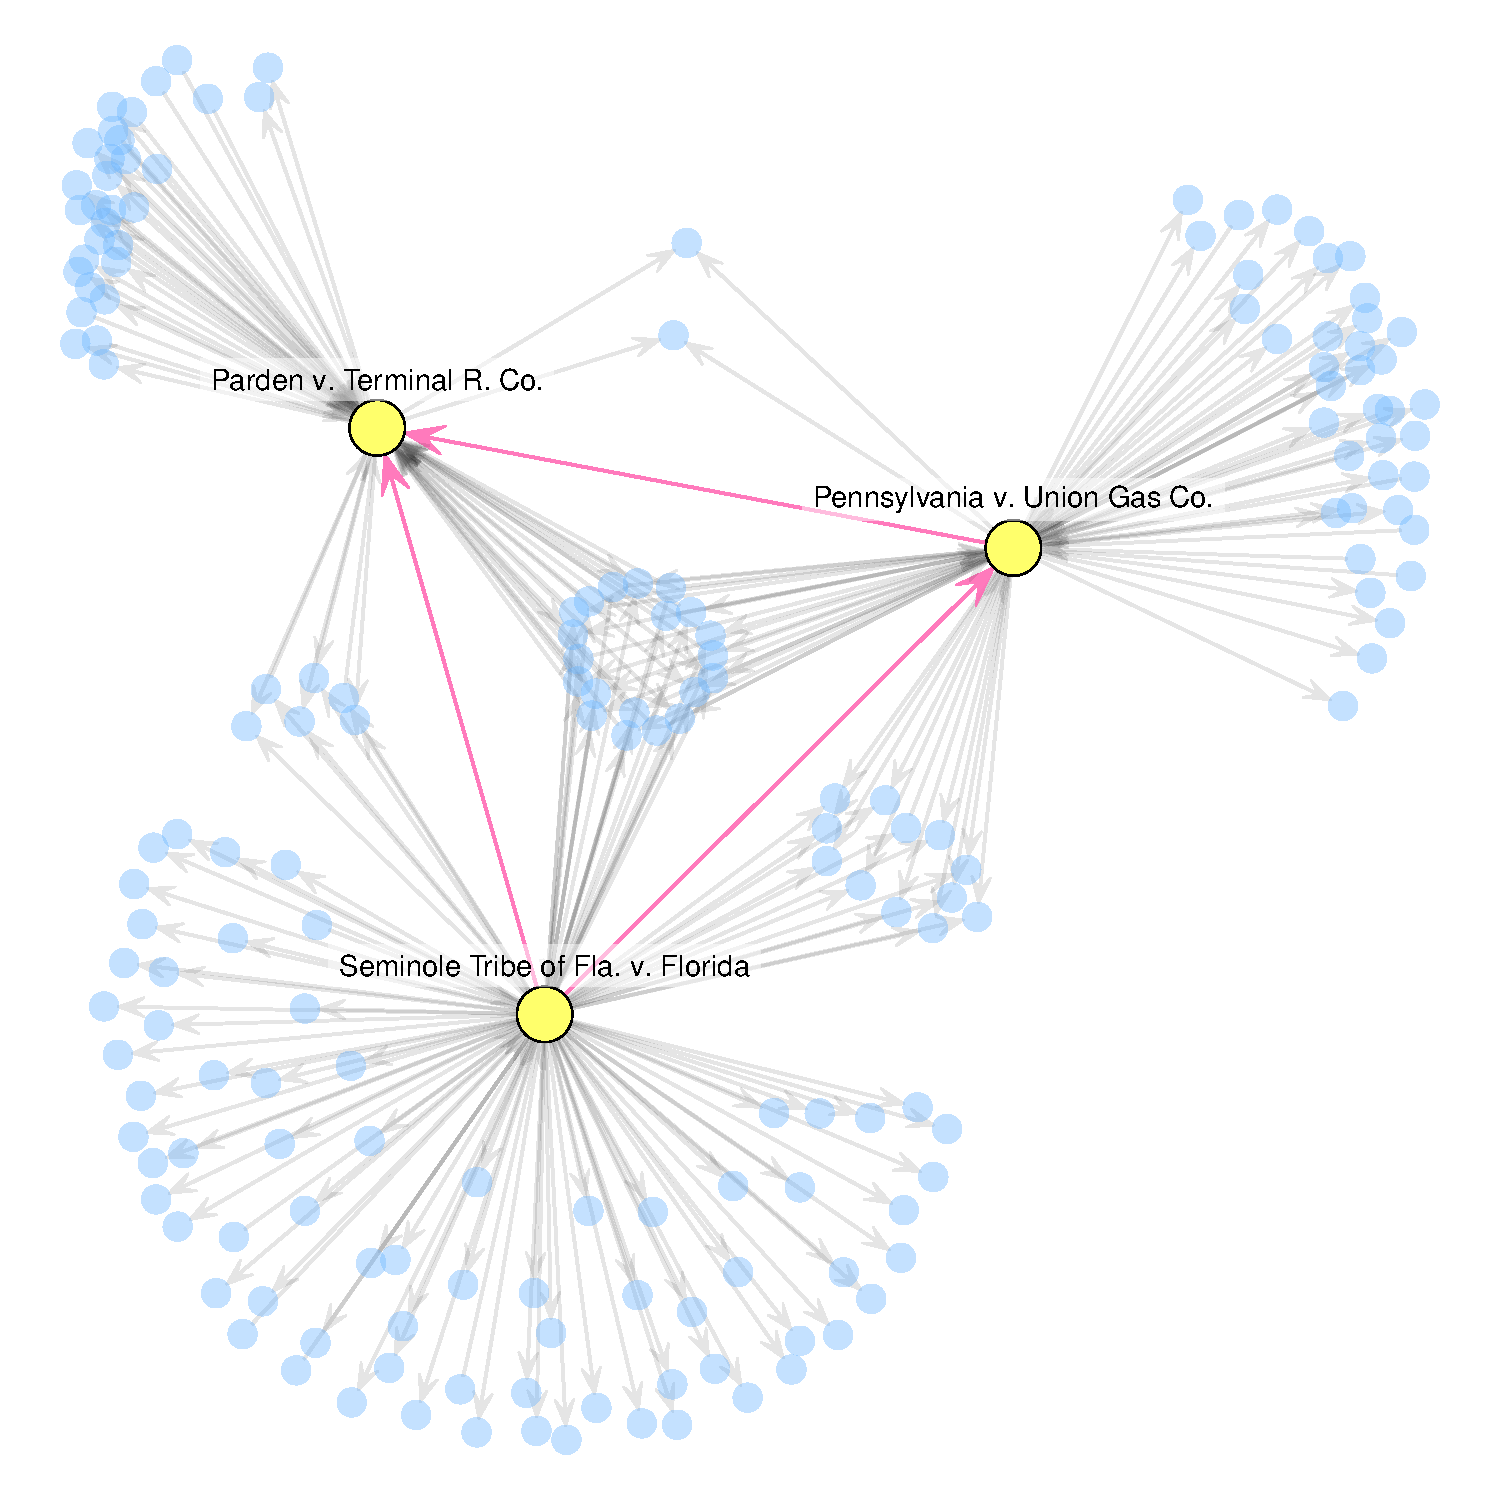
\includegraphics[width = 0.95\textwidth,trim= 0cm 1cm 0cm 2cm,clip=true ]{images/citations_trans.pdf}
\caption{Illustration of transitive triangle connecting US Supreme Court opinions through citations.}
\label{fig:transitivity}
\end{figure}

In the first example, a passage from Kansas v. Marsh (548 U.S. 163, 2006)---a case considering the constitutionality of a death sentence statute in Kansas. In this example, the case Stringer v. Black is cited by Kansas v. Marsh as a case that is quoted by Sochor v. Florida. The primary precedent under discussion in this passage of the opinion is Sochor v. Florida, but Stringer v. Black is cited as a result of its role in the Sochor v. Florida opinion.
\begin{quotation}
The statute thus addresses the risk of a morally unjustifiable death sentence, not by minimizing it as precedent unmistakably requires, but by guaranteeing that in equipoise cases the risk will be realized, by ``placing a `thumb [on] death's side of the scale,' '' Sochor v. Florida, 504 U. S. 527, 532 (1992) (quoting Stringer v. Black, 503 U. S. 222, 232 (1992); alteration in original).
\end{quotation} %https://supreme.justia.com/cases/federal/us/548/163/dissent2.html
The second example, which we illustrate visually in Figure \ref{fig:transitivity} is a passage from Seminole Tribe of Fla. v. Florida, 
(517 U.S. 44 1996)---a case addressing the rights of groups and citizens to sue states in federal court. In this example, Pennsylvania v. Union Gas Co
(491 U.S. 1, 1989) is the primary precedent being critiqued, and several cases are cited and discussed in terms of their roles as precedents in the Union Gas opinion. We highlight one---Parden v. Terminal R. Co., which is cited and discussed in both the Seminole and Union Gas opinions. 
\begin{quotation}
Never before the decision in Union Gas had we suggested that the bounds of Article III could be expanded by Congress operating pursuant to any constitutional provision other than the Fourteenth Amendment. Indeed, it had seemed fundamental that Congress could not expand the jurisdiction of the federal courts beyond the bounds of Article III. Marbury v. Madison, 1 Cranch 137 (1803). The plurality's citation of prior decisions for support was based upon what we believe to be a misreading of precedent. See Union Gas, 491 U. S., at 40-41 (SCALIA, J., dissenting). The plurality claimed support for its decision from a case holding the unremarkable, and completely unrelated, proposition that the States may waive their sovereign immunity, see id., at 14-15 (citing Parden v. Terminal Railway of Ala. Docks Dept., 377 U. S. 184 (1964)), and cited as precedent propositions that had been merely assumed for the sake of argument in earlier cases, see 491 U. S., at 15 (citing Welch v. Texas Dept. of Highways and Public Transp., 483 U. S., at 475-476, and n. 5, and County of Oneida v. Oneida Indian Nation of N. Y., 470 U. S., at 252).'
\end{quotation}% https://supreme.justia.com/cases/federal/us/517/44/case.html


The second network property we consider in the context of Supreme Court citations is reciprocity. Reciprocity (also referred to as mutuality) is the tendency for node B to send a tie to node A in response to or coordination with A sending a tie to B \citep{garlaschelli2004patterns}. It is typically not possible for reciprocated ties to form in legal opinions. Most citations reference past opinions that were issued before the citing opinion's case was even argued before the Court.  However, opinions written within the same Supreme Court term are often drafted in tandem, and can cite each other reciprocally.  Opinion A citing opinion B within the same term represents a signal that opinion B is relevant to the legal reasoning underpinning opinion A. Unlike the citations themselves, the applicability of legal rules or lines of reasoning across cases is not directed---if A is relevant to B, B is highly likely to be relevant to A. We expect opinions written within the same term to exhibit a high degree of reciprocity. Below we provide two example passages from opinions that illustrate the phenomenon of within-term reciprocity.  

\begin{figure}[ht]
\centering
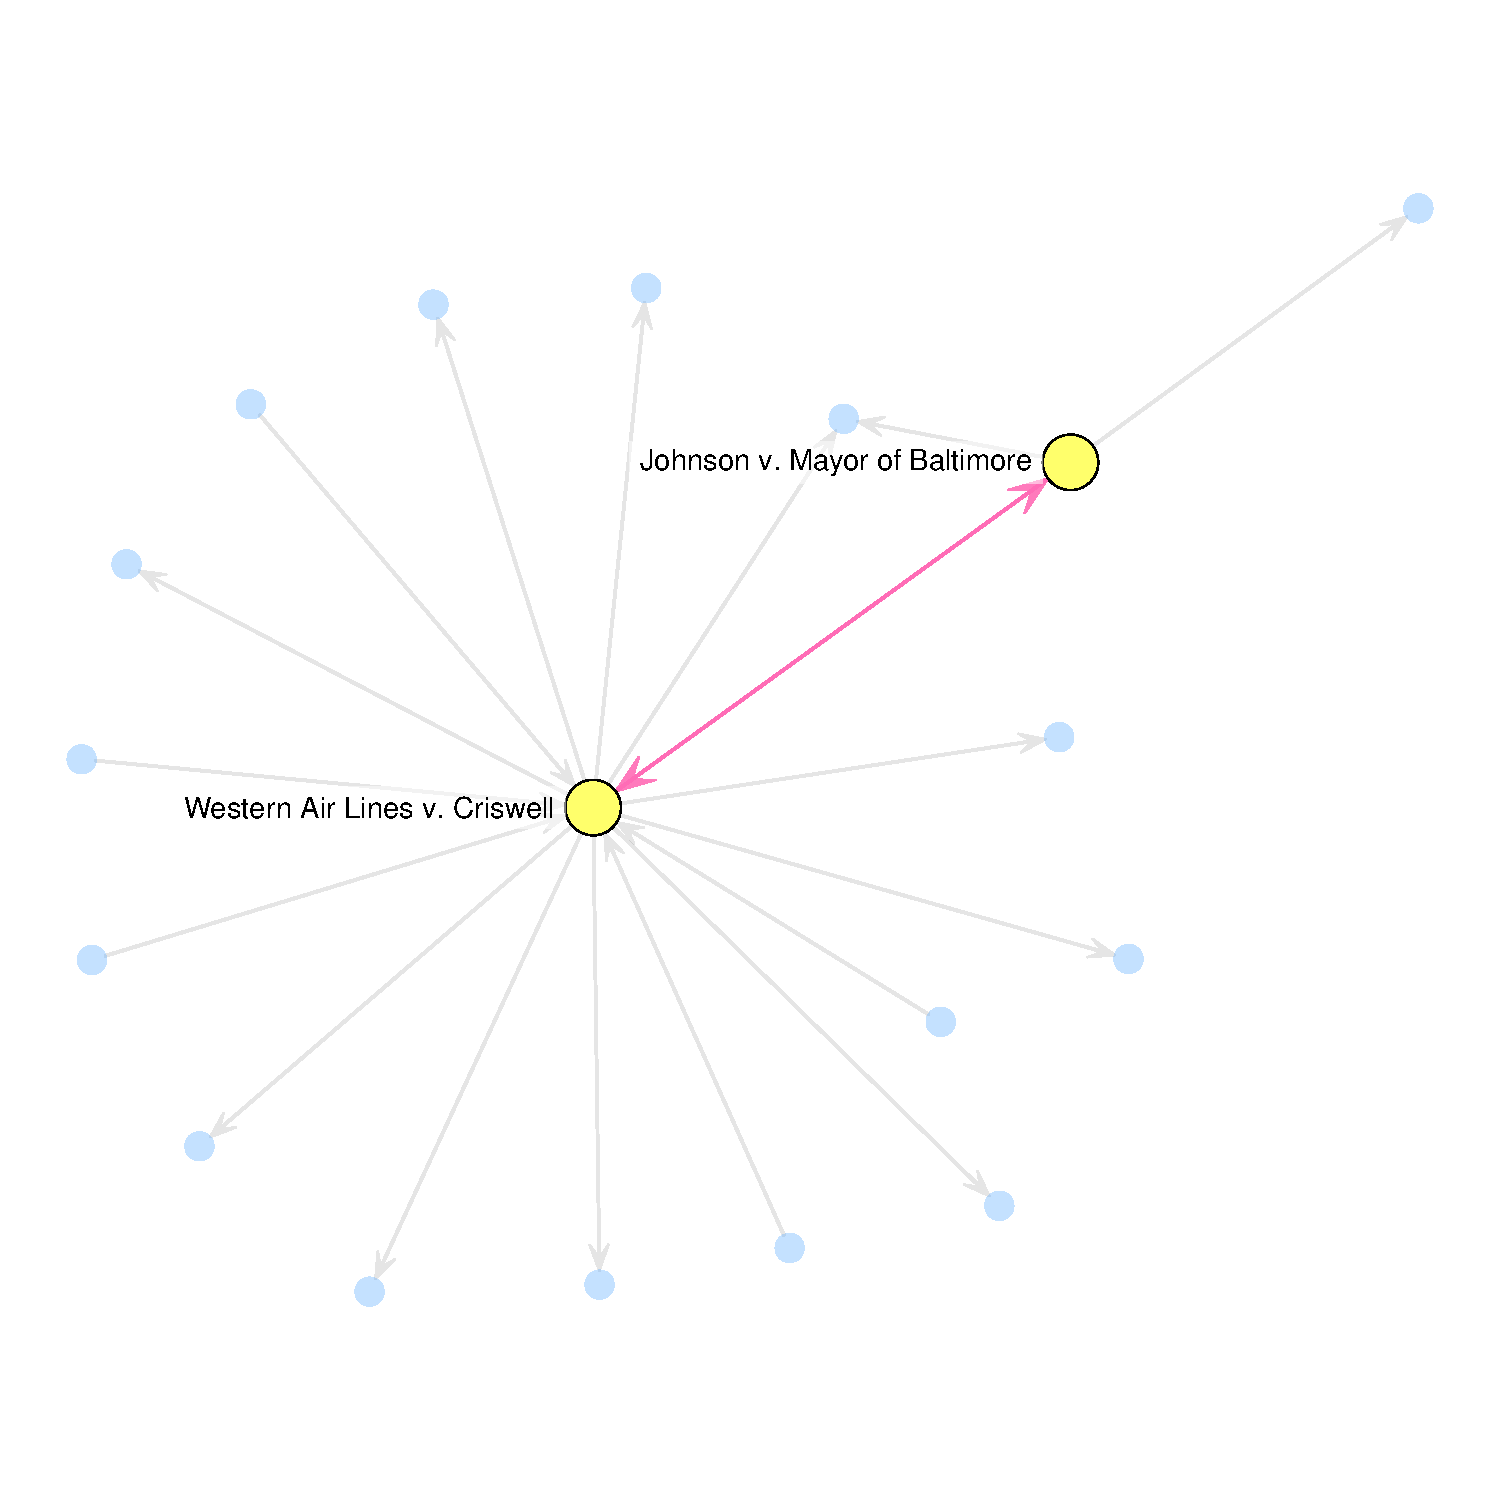
\includegraphics[width = 0.95\textwidth,trim= 0cm 1cm 0cm 2cm,clip=true ]{images/citations_recip.pdf}
\caption{Illustration of a reciprocal tie between two US Supreme Court opinions.}
\label{fig:reciprocity}
\end{figure}

The first case in our example reciprocal dyad is a passage from Western Air Lines v. Criswell (472 U.S. 400, 1985)---a case considering mandatory retirement in the context of age discrimination laws. The second case in the dyad, Johnson v. Mayor of Baltimore (472 U.S. 353, 1985) is another case considering whether mandatory retirement violates the Age Discrimination in Employment Act. The mutual edge connecting these two cases is visualized in Figure \ref{fig:reciprocity}. These cases addressed very similar legal questions, which increased the likelihood that they would inform each other, and the opinions were written within the same term, which made it possible for them to cite each other. 
\begin{quotation}
{\em From Western Air Lines:} On a more specific level, Western argues that flight engineers must meet the same stringent qualifications as pilots, and that it was therefore quite logical to extend to flight engineers the FAA's age 60 retirement rule for pilots. Although the FAA's rule for pilots, adopted for safety reasons, is relevant evidence in the airline's BFOQ defense, it is not to be accorded conclusive weight. Johnson v. Mayor and City Council of Baltimore, ante at 472 U. S. 370-371. The extent to which the rule is probative varies with the weight of the evidence supporting its safety rationale and "the congruity between the . . . occupations at issue." Ante at 472 U. S. 371. In this case, the evidence clearly established that the FAA, Western, and other airlines all recognized that the qualifications for a flight engineer were less rigorous than those required for a pilot.
\\~\\
{\em From Johnson:} The city, supported by several amici, argues for affirmance nonetheless. It asserts first that the federal civil service statute is not just a federal retirement provision unrelated to the ADEA, but in fact establishes age as a BFOQ for federal firefighters based on factors that properly go into that determination under the ADEA, see Western Air Lines, Inc. v. Criswell, post p. 472 U. S. 400. Second, the city asserts, a congressional finding that age is a BFOQ for a certain occupation is dispositive of that determination with respect to nonfederal employees in that occupation. 
\end{quotation} % https://supreme.justia.com/cases/federal/us/472/400/case.html \url{https://supreme.justia.com/cases/federal/us/472/353/case.html#370}

The third, and final, network property we consider in the context of Supreme Court citations is popularity. Popularity, also termed ``preferential attachment'' is the tendency for ties to be sent to nodes to which many ties have already been sent \citep{barabasi1999emergence}. Citations to an opinion signal both the Court's awareness of the legal reasoning of the case and the Court's evaluation that the opinion is an authoritative precedent. The more citations, the stronger this signal. Landmark cases, or those that establish new legal rules, are particularly authoritative and accrue citations from most future opinions that follow the respective line of reasoning. The passage below, from Oregon v. Mitchell (400 U.S. 112, 1970)---a case on the legality of state age restrictions on voting in federal elections---illustrates this popularity dynamic. In this opinion passage Baker v. Carr is cited in reference to its role as a landmark precedent, and noted for the number of other cases by which it has been followed. and for which an authoritative opinion is referenced, and even discussed in terms of the number of other cases by which it was followed. The language in this passage suggests that the attention to Baker v. Carr in previous Court opinions is in part responsible for its authority in Oregon v. Mitchell. The citations to Baker v. Carr are visualized in Figrue \ref{fig:popularity}.
\begin{quotation}
The first case in which this Court struck down a statute under the Equal Protection Clause of the Fourteenth Amendment was Strauder v. West Virginia, 100 U. S. 303, decided in the 1879 Term. [Footnote 2/1] In the 1961 Term, we squarely held that the manner of apportionment of members of a state legislature raised a justiciable question under the Equal Protection Clause, Baker v. Carr, 369 U. S. 186. That case was followed by numerous others, e.g.: that one person could not be given twice or 10 time the voting power of another person in a state-wide election merely because he lived in a rural area..."
\end{quotation} %https://supreme.justia.com/cases/federal/us/400/112/case.html

\begin{figure}[ht]
\centering
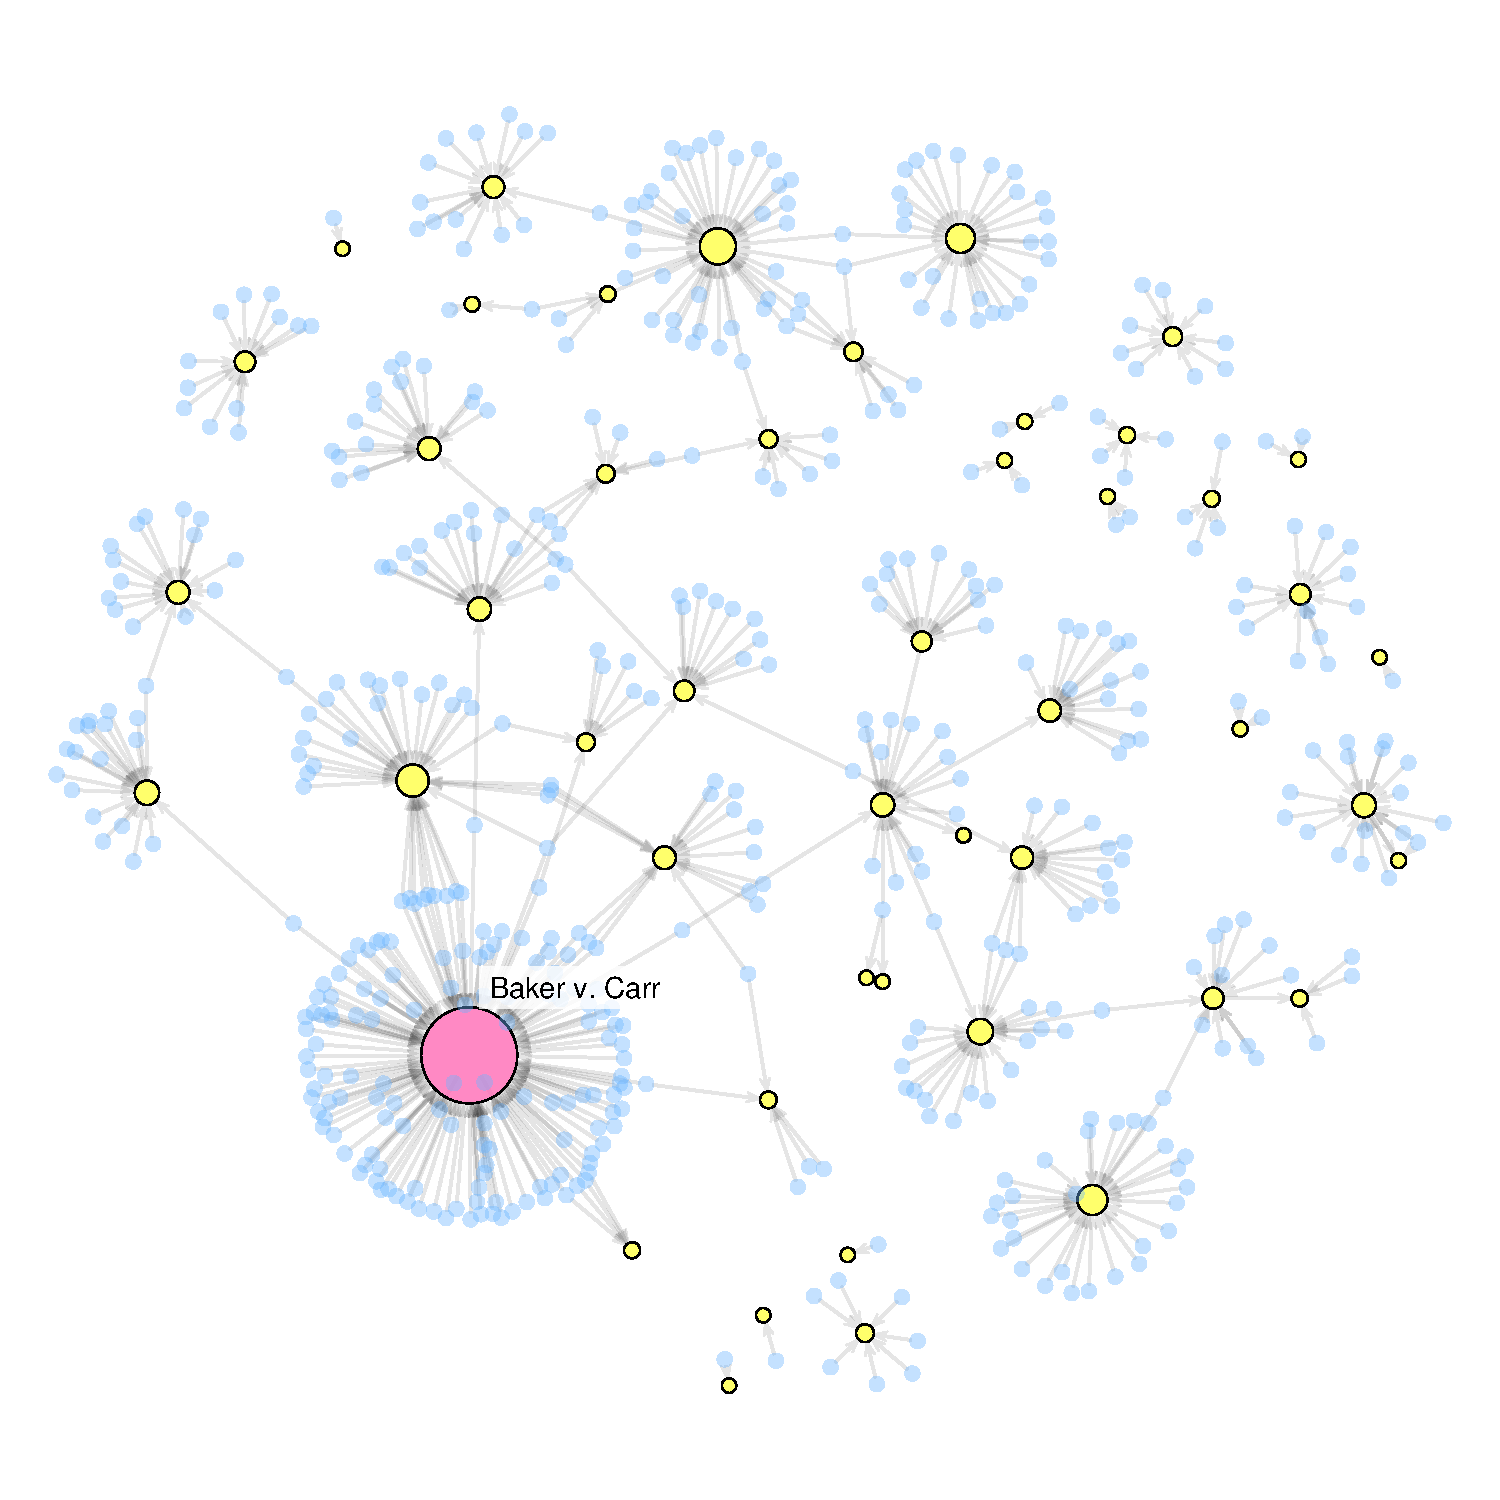
\includegraphics[width = 0.95\textwidth,trim= 0cm 3cm 6cm 8cm,clip=true ]{images/citations_pop.pdf}
\caption{Illustration of ties sent to a landmark Supreme Court opinion via citations.}
\label{fig:popularity}
\end{figure}

These three properties---transitivity, reciprocity, and popularity form the core of our network theory of U.S. Supreme Court citations. We also seek to model the effects of covariates (i.e., case features) on citation formation.  In the next section, we introduce a modeling framework that can incorporate all of these effects into a single model, and adapt to the peculiar structure of citation matrices.

 
\section{The Citation Exponential Random Graph Model}
We develop a methodology that can be used to jointly test for the effects of covariates on citations---as have been studied in prior research, and test for dependence effects, as we hypothesize above. To accomplish this, we extend a model that has been developed to jointly represent covariate and dependence effects in network data---the exponential random graph model (ERGM) \citep[e.g.,][]{duque2018recognizing,osei2018elite}.  %The ERGM, as it is currently implemented \citep{leifeld2017temporal,  tergm}, is designed to model longitudinal network data in which ties among a relatively stable set of nodes are modeled at multiple time points (e.g., the countries that are and are not defensively allied at time $t$, the legislators who have and have not cosponsored each others' legislation in the current session).  
The network structures for which ERGMs are currently designed are insufficient to account for the structure of citation networks.


We develop the citation ERGM (c-ERGM), to account for the structural constraints that apply to the network of Supreme Court citations. These structural constraints amount to three departures from the structure of networks for which ERGMs are currently designed. First, the citation network is partially acyclic. If two cases are decided during the same term, they can cite each other, forming a mutual edge (or two-cycle). However, if case $i$ is decided before case $j$, case $j$ can cite case $i$, but case $i$ cannot cite case $j$. Second, new edges can be created over time, but cannot be eliminated. Unlike in, e.g., an alliance network, in which two countries can dissolve an alliance, once a citation exists in a citation network it cannot be dissolved. Third, the set of nodes in the network must increase for new edges to be created. In conventional ERGMs, the number of nodes in the network can increase or decrease in each time period, and is typically stable over time. In a citation network, new edges (and non-edges) are introduced over time via the introduction of new nodes. The structure of the citation network is depicted in Figure \ref{fig:ctergm}---a hypothetical citation network established over three time periods, with three cases decided in each time period. We denote $C_t$ to be the set of citation and non-citations added to the network at time $t$ (i.e., via the addition of three cases), $C_{ <t}$ to be the citations among cases decided before time $t$, and $C_{ \leq t}$ to denote the entire set of citations and non-citations on which $C_t$ can depend through the c-ERGM specification.


\begin{figure}[H]
\centering
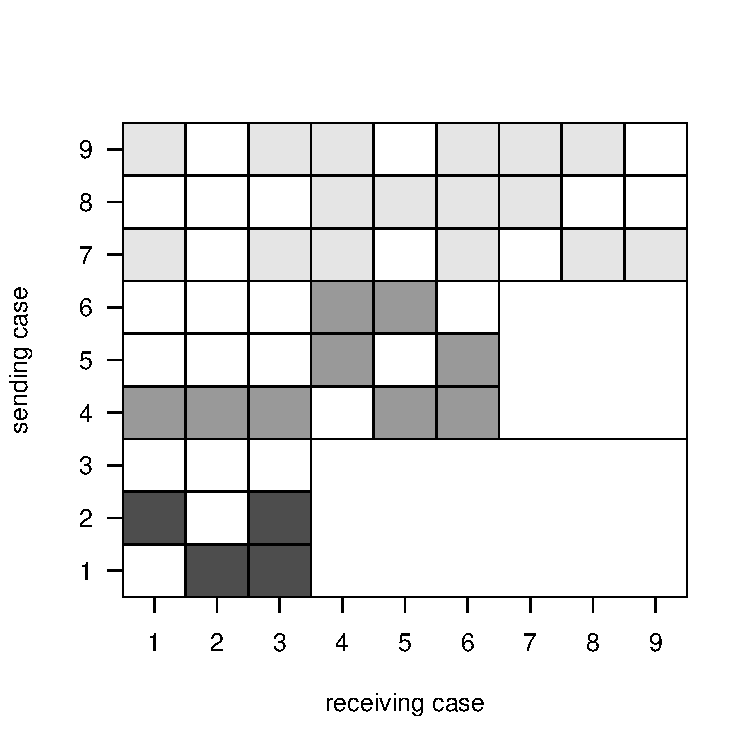
\includegraphics[width = 0.95\textwidth,trim= 0cm 0cm 0cm 0cm,clip=true  ]{images/daggish.pdf}
\caption{Illustration of temporal structure of the Supreme Court Citation Network. $C_{\leq t}$ is the entire set of citations (and non-citations) on which citations and non-citations at time $t$ (i.e., $C_t$) depend. $C_t$ are conditioned on the citations and non-citations established before time $t$ (i.e., $C_{< t}$). The shaded small squares are hypothetical observed citations, and the white small squares are citations that could have been observed but were not. The regions of the citation matrix that are represented by large white rectangles are citations that could not have been observed since the citing case would have been decided in a term that preceded the term of the cited case. The citing case ID is given in the row and the prospective cited case is given in the column. }
\label{fig:ctergm}
\end{figure}


The likelihood function of the c-ERGM is given by
\begin{equation}
l(\bm{\theta},C_{\leq t}) =  \frac{ \exp \left[ {\bm{\theta}'\bm{h}(C_{t},C_{<t}) } \right] }{ \sum_{C_t^* \in \mathcal{C}_t} \exp \left[ {\bm{\theta}'\bm{h}(C^*_{t},C_{<t}) }\right]  },
\end{equation}
where $\bm{\theta}$ is a vector of real-valued parameters, and $\bm{h}(C_{t},C_{<t})$ is a vector of scalar-valued functions that each quantify a feature of the citation network (e.g., the relationship between citation ties and a case attribute, the number of mutual edges in the citation network). $\exp \left[ {\bm{\theta}'\bm{h}(C_{t},C_{<t}) } \right]$ is a positive weight that is proportional to the probability of observing any particular form of the citations and non-citations added to the network at time $t$.  The denominator of Equation 1 represents a normalizing constant, in which the positive weight is summed over all possible configurations of $C_{t}$, from the network in which the cases added to the network at time $t$ send no citations at all, to the network in which the cases added at time $t$ cite every possible case, and everything in between. %The probability of observing the citation network up to time $T$---the final time point in the dataset---is given by the product over the probability of adding the citations at each time point $t$, conditional on the citations that were added to the network previously. 

Though the likelihood function of the c-ERGM may appear quite different from that of statistical models conventionally used in political science, analysis of the conditional probability of a single citation from case $i$ to case $j$ reveals that we can interpret the parameters similar to logistic regression coefficients. $$ P(C_{ij,t} = 1 | C_{-ij,t}, C_{ < t}) = \frac{\exp \left[ {\bm{\theta}'\bm{h}(C_{t},C_{<t}| C_{ij,t} = 1) } \right]}{ \exp \left[ {\bm{\theta}'\bm{h}(C_{t},C_{<t}| C_{ij,t} = 1) } \right] + \exp \left[ {\bm{\theta}'\bm{h}(C_{t},C_{<t}| C_{ij,t} = 0) } \right]}, $$ $$ \text{~~~~~~~~~~~~~~~~~~~~~~~~~~~~~~~} = \frac{1}{ 1 + \exp \left[ - {\bm{\theta}'\left(\bm{h}(C_{t},C_{<t}| C_{ij,t} = 1) - \bm{h}(C_{t},C_{<t}| C_{ij,t} = 0)\right)} \right]}, $$
where $C_{ij,t} = 1$ indicates that case $i$ cites case $j$, $C_{ij,t} = 0$ indicates that case $i$ does not cite case $j$, $C_{-ij,t}$ is the observed elements of $C_{t}$ except $C_{ij,t}$, and $\left(\bm{h}(C_{t},C_{<t}| C_{ij,t} = 1) - \bm{h}(C_{t},C_{<t}| C_{ij,t} = 0)\right)$ is the change in $\bm{h}(C_{t},C_{<t})$ that results from toggling $C_{ij,t} = 0$ to $C_{ij,t} = 1$. This re-arrangement illustrates that the parameters can be interpreted in terms of the change in the log odds of a citation from $i$ to $j$ given a one-unit increase in the corresponding element of $\bm{h}$, conditional on the other citations observed in the network. For example, if the value of $\theta$ corresponding to an element of $\bm{h}$ that counts the number of mutual edges in the network is 0.5, then the log odds of observing $C_{ij,t} = 1$ increases by 0.5 if case $i$ is cited by case $j$ (as compared to the configuration in which case $j$ does not cite case $i$). The logit form conditional probability is well known for the ERGM family \citep{goodreau2009birds}. Estimation of the c-ERGM parameters, which is done with a computationally-intensive, simulation-based approach, is presented in detail in the appendix.


%We should note that there is nothing about the c-ERGM (or any ERGM family model, for that matter) that permits the identification of causal effects of one tie on the formation of another. For example, if we find a positive popularity effect, the term for that dynamic would indicate that there is an increase in the log odds that case $i$ cites case $j$ with each other case that has cited case $j$.  That finding could be driven by one of two (or some combination of both) dynamics. First, it could be the case that a large volume of citations to a case in past opinions draws the attention of the justices to the ``popular'' case---as in the Baker v. Carr passage cited above. Second, it could be that we have omitted a case-level variable that is strongly associated with the number of citations accumulated by a case, and the number of citations in past cases is operating as a proxy for this unmeasured case characteristic. We cannot statistically differentiate between these two dynamics. However, in both of these conditions, and analogous conditions related to other dependence properties, citations (or non-citations) to a case are not independent conditional on the other variables, and the c-ERGM can be specified to account for the dependence in the data. Estimation of the c-ERGM parameters, which is done with a computationally-intensive, simulation-based approach, is presented in detail in the appendix.




%Methods of Monte Carlo approximation are well established in the ERGM literature, \citep{hunter2006inference,van2009framework,hummel2012improving}, but with a number of nodes on the order of $10,000$, even the methods of Monte Carlo MLE are computationally expensive \citep{schmid2017exponential}. However, because the network is large, we can rely on a fast estimation method---maximum pseudo-likelihood estimation (MPLE), which is consistent for discrete exponential family models \citep{nguyen2017near}, and has long been used with ERGM \citep{strauss1990pseudolikelihood}. The MPLE is defined as maximizing the log product of the conditional probability of each citation (and non-citation), conditional on the other elements of the observed citation network. The joint probability of all citations is replaced by the product over conditional probabilities, which, as we demonstrated above, assume a logit form. 

%One challenge that arises with the use of MPLE is that the usual estimate of the asymptotic covariance matrix (i.e., inverting the negated Hessian of the objective function at the maximum), results in standard errors that are biased downward. This leads to a high Type-1 error rate in hypothesis testing with MPLE if conventional standard errors are used \citep{van2009framework}. A form of non-parametric cluster bootstrap results in confidence intervals with correct coverage probability with MPLE \citep{desmarais2012statistical,desmarais2010consistent}. In the case of c-TERGM, the clusters are defined by $t$---the time points in which the cases are decided, and $T$ time-specific citation matrices $C_{t}$ are re-sampled with replacement to form a non-parametric cluster bootstrap sample. Confidence intervals are defined by the quantiles in the empirical distributions of estimates that result from re-estimating the MPLE on non-parametric cluster bootstrap samples. 


 \section{Empirical Analysis}
Our three data sources for this study include the Supreme Court Database (SCDB) \citep{spaeth2014supreme}, Martin-Quinn scores \citep{martin2002dynamic}, and Supreme Court citation data provided by the CourtListener Free Law Project \citep{CourtListener}. In the next section we explain the variables we construct using these data sources. We limit the Supreme Court terms included in our analysis to those that are covered by all three of these data source (1937--2015)\footnote{There were 145 cases that were listed in the SCDB but could not be matched to a case in the CourtListener data. We decided to exclude these 145 cases from our analysis. Additionally, since the most commonly used data on Supreme Court citations in political science come from \citet{fowler2007network}, we compared the Fowler data to the CourtListener data in the time interval that they overlap (1937--2001). We found considerable agreement---over 95\% of the citations recorded in the CourtListener dataset were also in the Fowler dataset, and over 96\% of the citations recorded in the Fowler data were also in the CourtListener dataset.}. The Supreme Court citation network from $1937 - 2015$ consists of $10,020$ cases. The breakdown of the data by the Court's Chief Justice is presented in Table \ref{tab:chiefs}. The network has a total of $112,939$ citation ties.\footnote{In order to focus on citation actions that were not intended to totally invalidate an opinion, we exclude $315$ citations that caused the cited case to be overruled. The data on overruling citation came from \citet{senate2016constitution}. Our results are virtually unchanged if we include the overruling citations.} The in- and outdegree distributions (i.e., the distributions of the number of citations sent and received by cases, respectively), are visualized in Figure \ref{degree_dist}. The maximum indegree (i.e., number of cases citing to a case) is $230$ and the maximum outdegree (i.e., number of cases cited by a case) is $162$. The majority of cases cite to and/or are cited by twenty or fewer other cases.

\begin{table}[htp]
\centering
\begin{tabular}{|
>{\columncolor[HTML]{C0C0C0}}l |l|l|l|}
\hline
{\color[HTML]{333333} } & \cellcolor[HTML]{C0C0C0}{\color[HTML]{333333} Terms} & \cellcolor[HTML]{C0C0C0}{\color[HTML]{333333} Total Number Cases} & \cellcolor[HTML]{C0C0C0}{\color[HTML]{333333} Cases/Term} \\ \hline
CE Hughes*              & 1937 - 1941                                          & 628                                                               & 125.6                                                     \\ \hline
HF Stone                & 1942 - 1946                                          & 756                                                               & 151.2                                                     \\ \hline
FM Vinson               & 1946 - 1953                                          & 789                                                               & 98.63                                                      \\ \hline
E Warren                & 1954 - 1969                                          & 2149                                                              & 126.41                                                     \\ \hline
WE Burger               & 1970 - 1986                                          & 2805                                                             & 155.83                                                     \\ \hline
W Rehnquist            & 1987 - 2005                                          & 2022                                                              & 106.42                                                      \\ \hline
J Roberts **           & 2006 - 2015                                          & 871                                                              & 87.1                                           \\ \hline
\end{tabular}
\caption[caption]{For the time range of interest (1937 - 2015) this table displays the chief justices, the time range they served as chief justice, the number of cases in their time range as well as the average number of cases per year.\\\hspace{\textwidth} * CE Hughes served as chief justice from 1930 - 1941. \\\hspace{\textwidth} ** J Roberts still serves as chief justice (retrieved 5/2020).}
\label{tab:chiefs}
\end{table}


The degree distributions indicate that there is a long tail to both the number of citations sent and received. These long-tailed (i.e., high kurtosis) distributions provide preliminary evidence of substantial heterogeneity in the features that drive citations to and from cases \citep{strogatz2001exploring}. Figure \ref{fig:networkviz} displays the citation network network from 1937--2001. We see here that the densest rates of tie formation tend to be between consecutive courts (e.g., the Stone Court is much more tightly tied to the Hughes Court than the Rehnquist Court is to the Hughes Court). This pattern lends preliminary/descriptive support to the hypothesis that the rate of citations to a case decrease over time.


\begin{figure}[H]
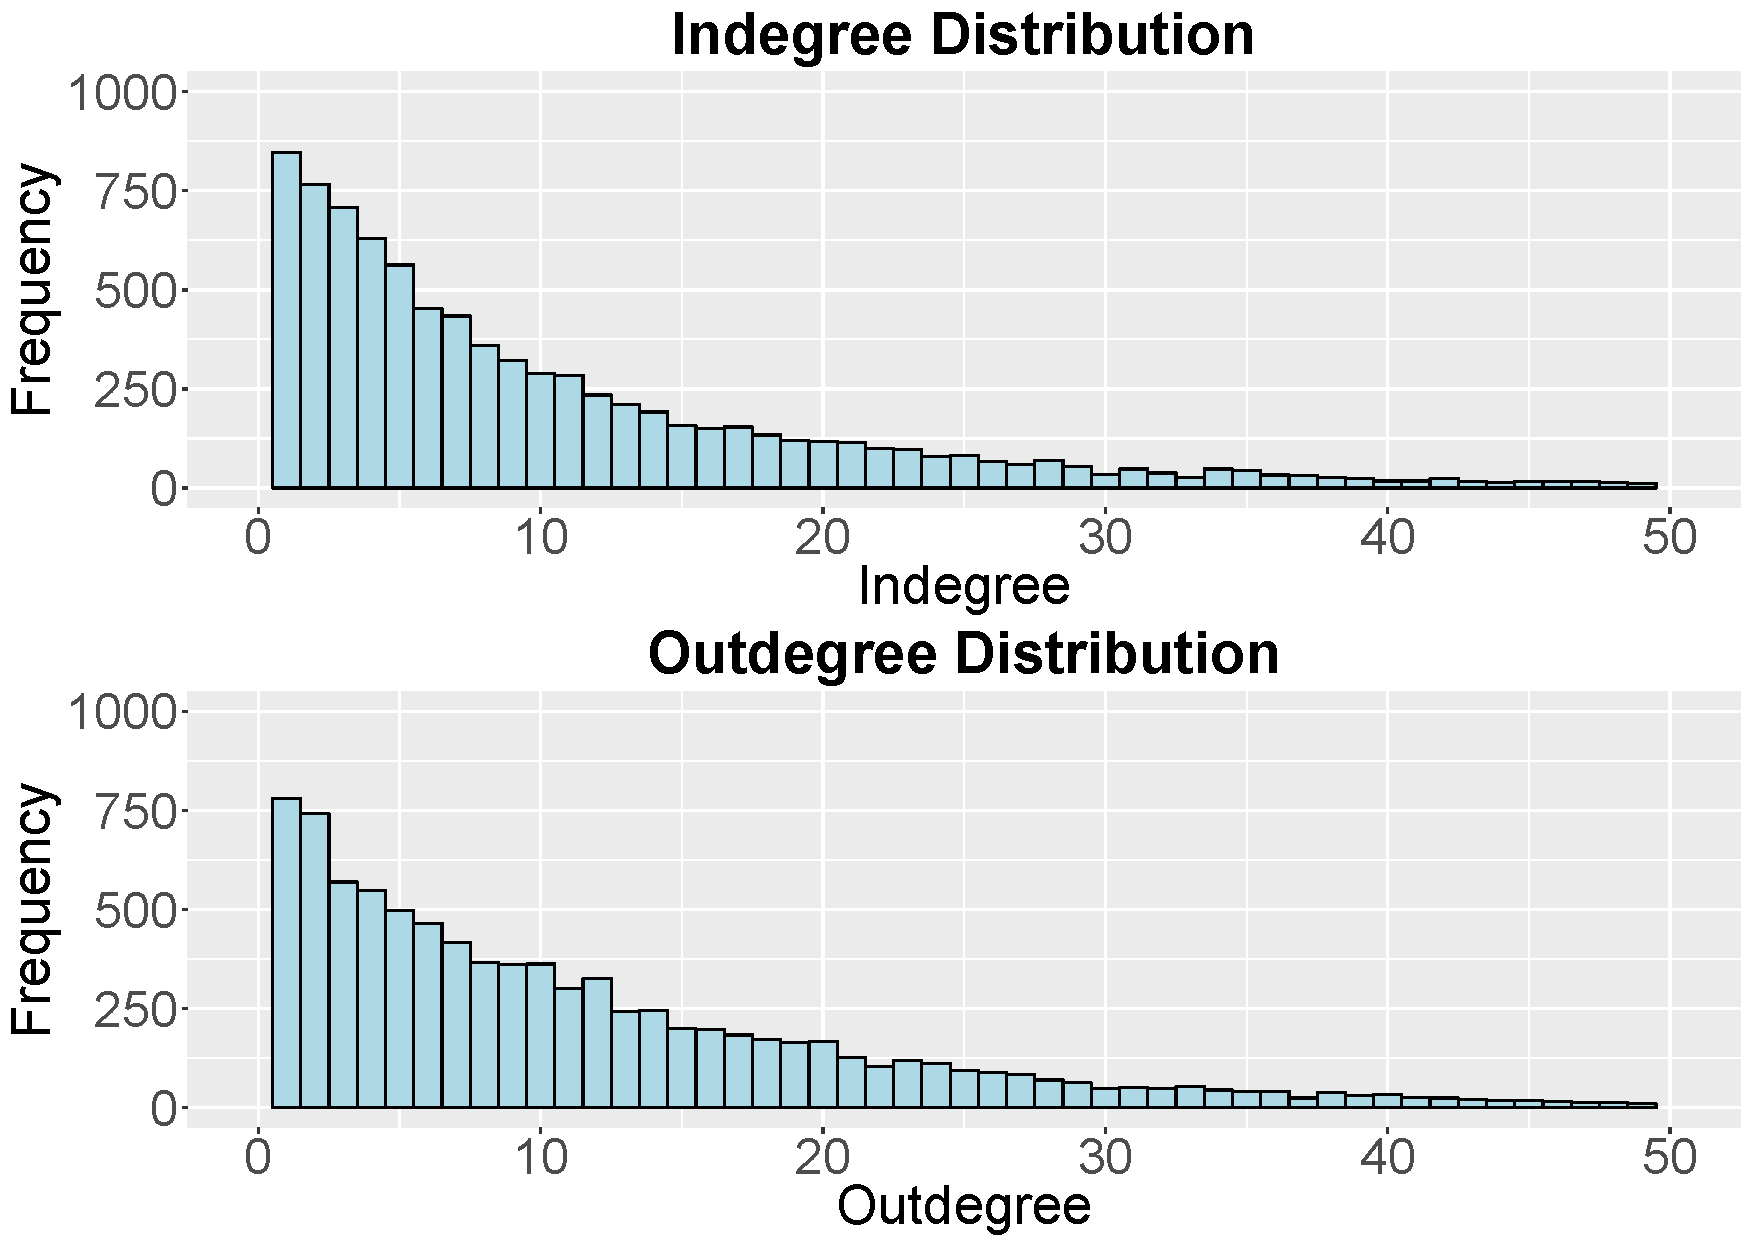
\includegraphics[scale=0.5]{degree_distribution}
\caption{The in- and outdegree distribution of the Supreme Court Citation Network from 1937 - 2001. There are cases with an indegree  $>$50, but they are not captured in this figure.}
 \label{degree_dist}
\vspace{-.25cm}
\end{figure}

\begin{figure}[H]
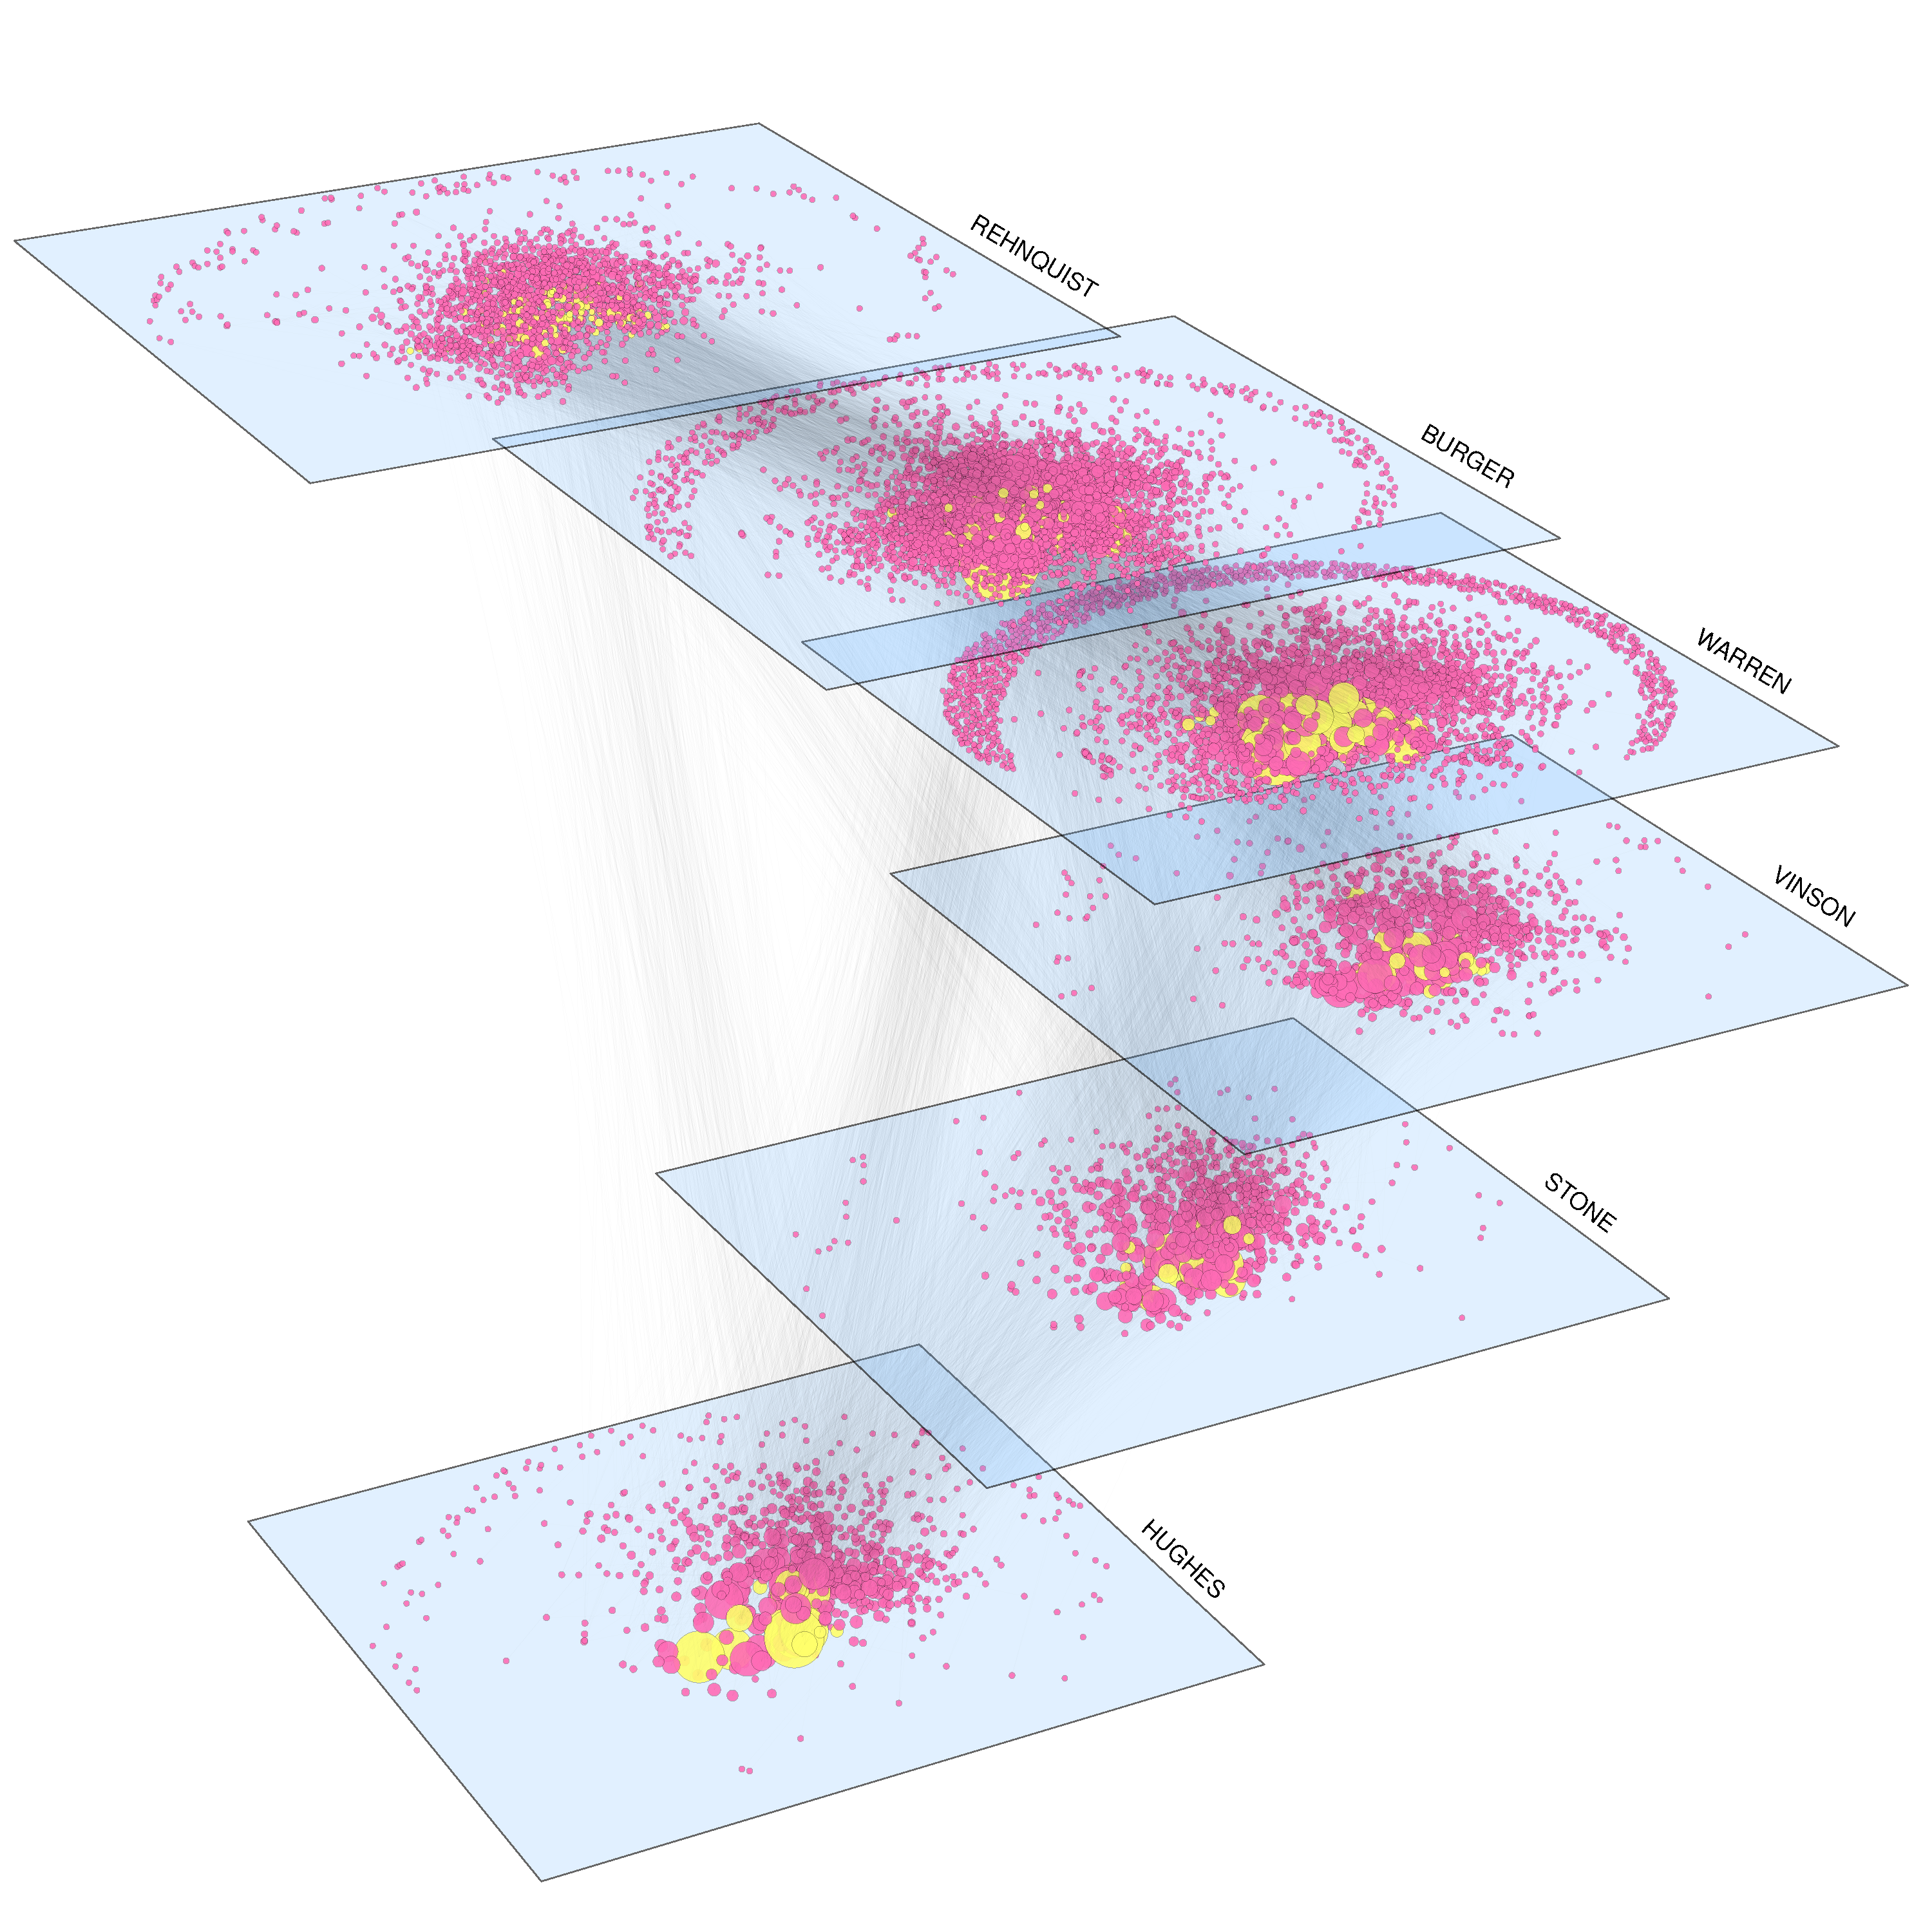
\includegraphics[scale=0.35,clip=true,trim=.5cm 0cm 0cm 2cm]{images/citations1}
\caption{ Supreme Court Citation Network, 1937-2001. Nodes are Supreme Court cases, with size based on incoming citations. Salient cases ({\em Oxford Guide}) are in yellow. Each network layer contains cases decided under a different chief justice. Because our data is temporally bound, cases for the Hughes and Rehnquist courts are not complete. }
 \label{fig:networkviz}
\vspace{-.25cm}
\end{figure}


\subsection{c-ERGM specification}

The c-ERGM we estimate includes two classes of terms---one that captures the effects of covariates on tie formation, and another that captures the complex dependence processes that we expect to observe in the Supreme Court Citation Network. We describe our model specification by defining the terms within these two classes.


\subsubsection{Covariate terms}\label{covariate_terms}

Covariate effects are accounted for in the c-ERGM via the term that is used to specify the effect of covariates in other ERGM family models, as
$$h_{covariate}(C_t,C_{<t},X) =  \sum_{ij} C_{ij,t}X_{ij}.$$ Since $C_{ij,t}$ is a binary indicator of whether case $i$ cites case $j$, $h_{covariate}$ amounts to the sum of covariate values among directed dyads for which we observed a citation. The dyadic interpretation of the coefficient attributed to this term is the change in the log odds of a tie from $i$ to $j$ given a one-unit increase in $X_{ij}$ (i.e., exactly the interpretation of the effect of a covariate in logistic regression). We include several exogenous covariates based on this standard formulation. 

The first covariate we incorporate into the model accounts for the degree to which cases cite those that are similar in terms of the ideological positions of the justices who supported the decision. We account for this effect following \citet{spriggs2001explaining}, who find that cases are more likely to be overruled when the Court is ideologically distant from the median justice in the majority coalition that decided the case. \citet{clark2010locating} estimates a latent coordinate model of Supreme Court opinions based on the network of case-to-case citations. They find that the majority opinion falls at the ideal point of the median member of the majority coalition in the case. We include a covariate term in which $X_{ij}$ is the absolute difference between the Martin-Quinn scores \citep{martin2002dynamic} of the median justices in the majority coalitions for cases $i$ and $j$. We expect this variable to have a negative effect, which would correspond to cases citing those to which they are ideologically similar. %WE COULD USE THIS DATASET AS A SECOND APPLICATION


%We include three sets of dummy variables that account for the issue areas of cases. In the first set of dummy variables---sender intercepts---the variable $X^{ij}$ indicates the issue area of the sending case ($i$) (e.g., for the Criminal Procedure indicator, $X_{ij} = 1$ if case $i$ is a criminal procedure case, and $0$ otherwise). The second set of dummy variables represent receiver issue area intercepts in which $X^{ij}$ indicates the issue of the receiver case. The third set of dummy variables account for the rate of citation within each issue area and between each combination of issue areas.  There is a separate dummy variable for each directed pair of issue areas. For example the A$\rightarrow$B dummy variable $X_{ij} = 1$ if case $i$ is issue area A and case $j$ is issue area B, and 0 otherwise. Note that, given the high dimension of these dummy variables, we omit one each of the sender and recipient indicators, and 28 of the 196 mixing rate indicators. Unfortunately, this leaves these indicators largely uninterpretable, but these variables are nonetheless important to absorb variation in citations that is attributable to the legal domains of two cases in a dyad. The Issue area data comes from the Supreme Court Database (SCDB) \citep{spaeth2014supreme}. We include these variables because \citet{cross2010determinants} finds that the number of citations to Supreme Court opinions depends heavily on the issue area of the case. Table \ref{issue_area_coding} reports the issue areas covered in our data.

We include one covariate that accounts for the rate at which cases that fall under the same issue area cite each other. The variable $X^{ij}$ indicates whether cases $i$ and $j$ share the same issue area, e.g., $X^{ij}=1$ if cases $i$ and $j$ are classified into the same issue area, and $0$ otherwise. The Issue area data comes from the Supreme Court Database (SCDB) \citep{spaeth2014supreme}. We include these variables because \citet{cross2010determinants} finds that the number of citations to Supreme Court opinions depends heavily on the issue area of the case. Table \ref{issue_area_coding} reports the issue areas covered in our data.

%We also include a set of covariates that account for justice-specific variation in citations. We include two types of terms at the justice level. First, we include an indicator variable that models the rate at which justices cite themselves. This effect is modeled with a single indicator variable in which $X_{ij} = 1$ if the majority opinions in cases $i$ and $j$ were written by the same justice. Second, we use two sets of dummy variables to account for differences across justices both in terms of their tendencies to include citations in the opinions they write and to be cited by other opinions. The justice sender dummy variables indicate the identity of the justice who authored the majority or plurality opinion of case $i$. The justice recipient dummy variables indicate the identity of the justice who authored the majority or plurality opinion of case $j$. This set of variables is motivated by the use of citations by \citet{kosma1998measuring} to measure the influence of individual Supreme Court justices.

We also include an indicator variable that models the rate at which justices cite themselves. Similar to the same issue area variable, this effect is modeled with a single indicator variable in which $X_{ij} = 1$ if the majority opinions in cases $i$ and $j$ were written by the same justice. The data is taken from the SCDB \citep{spaeth2014supreme}. 

\begin{table}[]
\centering
\begin{tabular}{llll}
1 & Criminal Procedure & 8  & Economic Activity    \\
2 & Civil Rights       & 9  & Judicial Power       \\
3 & First Amendment    & 10 & Federalism           \\
4 & Due Process        & 11 & Interstate Relations \\
5 & Privacy            & 12 & Federal Taxation     \\
6 & Attorneys          & 13 & Miscellaneous        \\
7 & Unions             & 14 & Private Action      
\end{tabular}
\caption{Assigned numbers for the variable \textit{Issue Area}. This information originates from the Supreme Court Database code book.}
\label{issue_area_coding}
\end{table}

We model the way in which citations to a case depend upon the age of a case. For this we use a second-order polynomial in which one covariate $X^{ij}$ is defined as the age of case $j$ at the time that case $i$ is decided, and another term in which $X^{ij}$ is the squared age of case $j$ at the time that case $i$ is decided. We include these covariates because \citet{black2013citation} find that the number of citations to a Supreme Court case over time depends significantly on the age of the case, characterized by a sharp drop off and leveling out with age. 

\citet{benjamin2012standing} study the propensity for cases to be overruled and cited in other negative ways. They find that cases with majority coalitions that are large and ideologically broad are less likely to be cited negatively. In our data we do not differentiate between negative and positive citations, but since the overwhelming majority of citations are positive, we hypothesize that the effects they found will be reversed in our analysis. We include one covariate in which $X^{ij}$ is the number of justices in the majority coalition for case $j$. We also include another covariate in which $X^{ij}$ is the absolute difference between the maximum and minimum ideal points of the justices in the majority coalition for case $j$. We expect both of these covariates to have positive effects.

The final control variable we include in the model is one in which $X_{ij} = 1$ if case $j$ was overruled prior to the term in which case $i$ was decided. This variable, quite simply, models the effect of being overruled on the rate of citation to a case after the overruling citation. \citet{fowler2008authority} find that citations to a case drop off quickly after the case has been overruled.


\subsubsection{Dependence terms}\label{dependence_terms}

We include dependence terms to account for each of the dynamics that we hypothesize will characterize the Supreme Court Citation Network---transitivity, reciprocity, and popularity. %We expect that the coefficients associated with each of these dependence effects will be positive. 

The common dependence effects for these three dynamics are the number of triangles (case $i$ cites cases $j$ and $k$, and case $j$ cites case $k$), the number of mutual dyads (case $i$ cites $j$ and vice versa), the number of out-2-stars (case $i$ cites $j$ and $k$), and the number of in-2-stars (case $i$ is being cited by cases $j$ and $k$) in $C_{\leq t}$. Unfortunately, adding the triangle, out-2-star, or in-2-star statistic causes model degeneracy \citep{Handcock.2003}. Model degeneracy is a common obstacle when fitting ERGMs, and occurs when the model places most of its probability mass on just a few networks, usually the empty and the full network. In this scenario, the simulated networks are too different from the observed network, making the underlying distribution defined by the model extremely unrealistic.

% reciprocity
The statistic included in the model for reciprocity counts the number of mutual dyads (i.e., dyads in which cases $i$ cites case $j$, and case $j$ cites case $i$) in $C_{\leq t}$. In practice, this is the number of mutual dyads in $C_{\leq t}$, since mutual dyads must emerge among opinions that were written in the same term. The log odds interpretation of the reciprocity statistic is that if the opinion in case $i$ cites case $j$, the log odds that case $j$ also cites $i$ change by the estimated coefficient relative to the configuration in which case $j$ does not cite case $i$. We expect the reciprocity effect to be positive.

% popularity
Accounting for the popularity effect through the in-2-star statistic is prone to cause model degeneracy. In an attempt to stabilize the model against model degeneracy as well as to still capture the popularity effect, \citet{SnijdersTomA.B..2006} introduces the \textit{alternating-in-k-star} statistic, which was shown to be equivalent to the \textit{geometrically weighted indegree distribution} (gwidegree) statistic introduced by \citet{hunter2006inference}. Define $D_r(C_t, C_{<t})$ as the number of nodes with indegree $r, r \in \{0, \dots , N_t -1 \}$, where $N_t$ is the number of cases in the network at time $t$, then gwidegree represents a network's indegree distribution in a single statistic by geometrically weighting the degree distribution
\begin{equation}
h_{gwidegree}(C_{t}, C_{<t}, \lambda)= \lambda \sum_{r=1}^{N_t-1}\biggl(1-\bigl(1-\frac{1}{\lambda}\bigr)^r\biggr)D_r(C_t, C_{<t}). 
\label{gwidegree}
\end{equation}
The decay parameter $\lambda \in [0, \infty ]$ controls the decline of the weight put on $D_r(C_t, C_{<t})$ as $r$ increases, which means that the higher $\lambda$ the more the statistic responds to changes for cases with a high indegree. We fixed $\lambda=1$. Adding one single edge to the network changes the indegree distribution of the network so that a case with an indegree of $s$ turns into a case with an indegree of $s + 1$. With our notation this means that $D_r$ and $D_{r+1}$ get replaced by
$D_r -1$ and $D_{r+1} +1$, while no changes for $D_\ell,
 \ell \in \{0, \dots , N_t -1 \} \setminus \{r, r-1\} $ are
made. This changes the log odds in the following way
$$\text{logit} P(C_{ij,t}=1 | C_{-ij,t}, C_{<t}) = \exp \bigl(~\theta \cdot( 1- \frac{1}{\lambda})^r \bigr).$$
As stated by \citet{Levy2016}, this means for the interpretation that a negative parameter value indicates the centralization of edges (i.e., popularity) while a positive parameter indicates the dispersion of edges (i.e., new ties going to less popular nodes). Since we expect highly cited cases to be more likely to be cited again, we expect the gwidegree parameter to be negative.


% Transitivity
We include two statistics to account for different types of transitivity.
The first transitivity statistic calculates the number of transitive ties, $i \to j$, where there is a directed path of length two from $i$ to $j$ through at least one case $k$, and $j$ and $k$ were written during a different term than $i$. We will refer to this statistic as the \textit{different term transitivity} statistic. As illustrated in Section 2, we theorize Supreme Court citations to pattern a high degree of transitivity. As a result, we expect positive parameter estimates for the \textit{different term transitivity} statistic. 


The second transitivity statistic, intended to capture clustering that includes more than one tie formed in the same term, is the \textit{geometrically weighted edgewise shared partners} (gwesp) statistic introduced by \citet{hunter2006inference}. For directed networks the edgewise shared $r$-partners statistic ($ESP_r$) can take multiple forms, but we integrate the definition where cases $i$ and $j$ that are connected by a citation, also cite $r$ common other cases. We follow the notation of \citet{Butts.2008} and call this ESP specification \textit{outgoing shared partners} (OSP). Similar to the gwidegree-statistic the gwesp-statistic incorporates a network's edgewise shared partners distribution by replacing $D_r$ by $ESP_r$. We fix the decay parameter at $\lambda=0.25$. Triangles that are incident to the outgoing shared partners configuration arise when there is a cite between two cases decided at the same time, and those two cases cite one or more of the same third cases (decided either previously or also during the same term). This would happen if citations were clustering around legal issues that are not completely captured by our same-issue-area effects.  As we do not expect that the issue area variable will account for all of the clustering around legal issues, we expect the gwesp statistic to also carry a positive coefficient value.

% Activity
We include one more structural network effect to adjust for inherent differences across cases in terms of the overall scope of the legal issues addressed in a case.  \citet{fowler2008authority} finds that cases vary in the degree to which they serve as ``hubs''---citing to many other cases. We expect that new cases will be more likely to cite cases that themselves cited many cases, because cases that themselves cite a large number of cases address a broader array of legal issues. We include the outdegree of every node that entered the network prior time $t$ as a receiver effect. We expect the coefficient on this term to be positive. This is not technically a dependence term, as it is formulated as a covariate, but we discuss it in the current section because it is purely a network structure effect.




%In order to account for the popularity effect, we add the \textit{geometrically weighted indegree distribution} (gwidegree) statistic to the model. The geometrically weighted distribution statistics were introduced by \citet{Hunter.2006} to counteract model degeneracy.




%The log odds interpretation of the triangle statistic is that  $\theta$ gives the change in the log odds of case $i$ citing case $j$ associated  with each additional triangle that would be created by case $i$ citing case $j$ (e.g., if opinions in cases $i$ and $j$ cite one common case $k$, the log odds that case $i$ cites case $j$ change by theta relative to the configuration in which cases $i$ and $j$ do not cite any of the same cases).


 % \subsubsection{Dynamics in effects}

% For the current model this section is not relevant anymore  
  
  
\subsection{Model Fit}

Our case for studying legal citations at the directed dyadic level hinges upon the contribution to modeling offered by incorporating network dependence. To quantify this contribution, we fit one model that incorporates covariate effects only, which we term the {\em Independent Model}---excluding the reciprocity, transitivity, and popularity terms. The full model is the one we present below. We use both AIC and BIC to compare the fit of the two models, with lower values indicating better fit.  

  \begin{figure}[H]
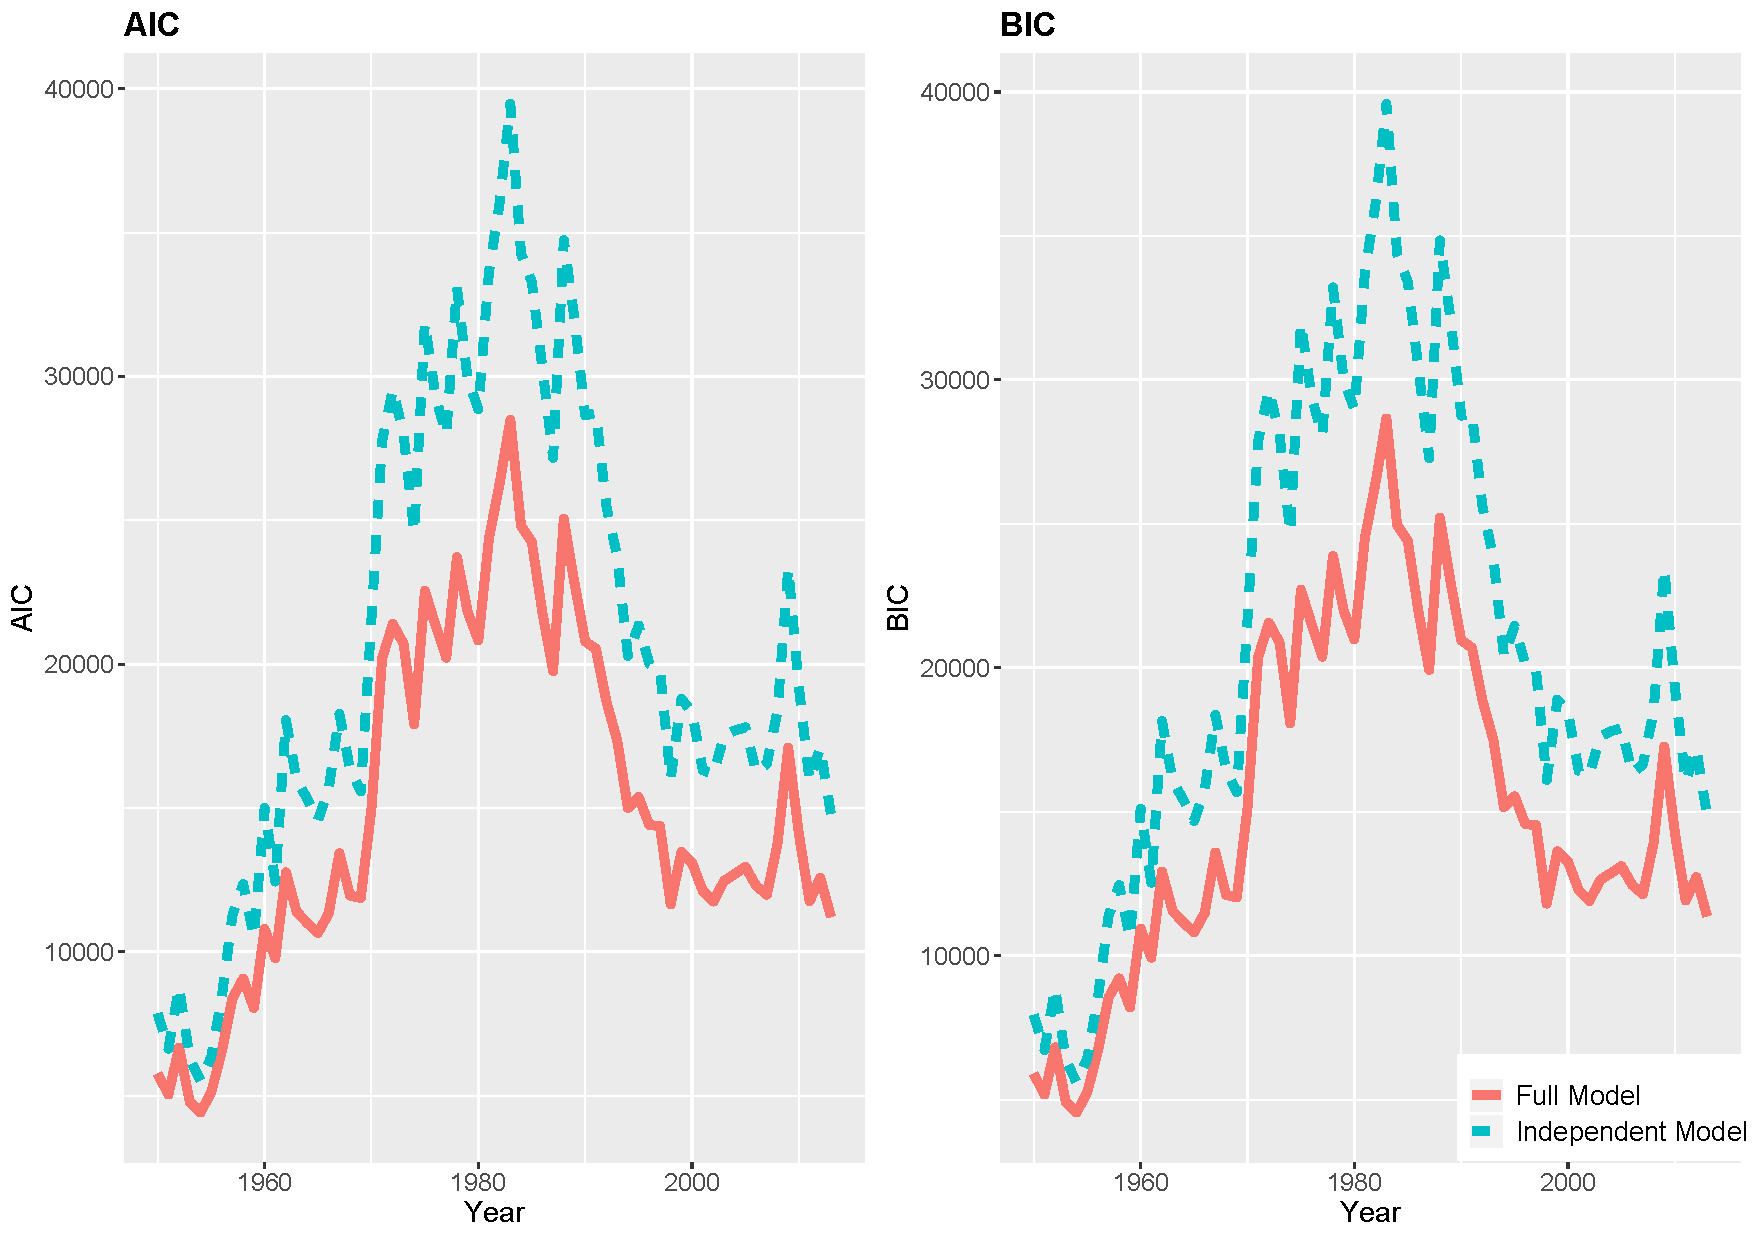
\includegraphics[width=15cm]{SCC_AIC_BIC}
\caption{AIC and BIC for the full and the independent model for the time frame 1950-2015 }
 \label{AIC_BIC}
\vspace{-.25cm}
\end{figure}  

Figure \ref{AIC_BIC} depicts the AIC and BIC comparison for the two different models for each term from 1950 to 2015. We see that the AIC and BIC is considerably smaller for the full model throughout the period of consideration. On average the independent model yields a 5,525 point higher AIC and an average 5,582 point higher BIC. The maximum difference is reached in 1983 with a difference of 10,990 points for the AIC and 10,930 points for the BIC. This fit comparison provides robust evidence that the dependence terms contribute significantly to the explanatory power of the model.\footnote{In the appendix we present conventional goodness-of-fit plots that are used to assess the structural fit for ERGM \citep{hunter2008goodness}, as well as degeneracy diagnostics \citep{mukherjee2020degeneracy}. We find that the full model fits the degree and edgewise shared partner distributions well, and is not degenerate.} 

%In our prediction experiment we randomly split the directed dyads into an 80\% training set and a 20\% test set. The parameters of the model are estimated using the directed dyads in the training set, and the parameters are used to form the conditional probability of a tie for all of the directed dyads in the test set. Directed dyads for which the conditional probability of a tie exceeds 0.5 are predicted to be citations. The experiment is run with the full model, and with a model that excludes all of the dependence terms (i.e., all terms involving reciprocity, in and out stars, and triangles)---the independent dyads model. We run this experiment for 10 iterations. Predictive performance is evaluated with three common and related measures---precision (i.e., the proportion of predicted citations that are actually citations), recall (the proportion of actual citations that are predicted to be citations), and the F1 score (the harmonic mean of precision and recall) \citep[see, e.g.,][for discussion of these measures]{makhoul1999performance}. All three measures are bounded between 0 and 1, with higher scores indicating better performance.

%\begin{table}[H]
%\centering

%\begin{tabular}{rllll}
%\hline \hline
%& \multicolumn{2}{l}{Independent Model } & \multicolumn{2}{l}{Full Model} \\ \hline 
% & mean & range & mean & range \\ 
%  \hline
%precision & 0.6007 & (0.5934, 0.6074) & 0.8666 & (0.8647, 0.8701) \\ 
%  recall & 0.1522 & (0.1495, 0.1549) & 0.5969 & (0.5945, 0.6019) \\ 
%  F1 score & 0.2429 & (0.2389, 0.2462) & 0.7069 & (0.7048, 0.7107) \\ 
%   \hline \hline
%\end{tabular}
%\caption{The predictive performance of the directed dyadic models with linear trends, over ten 80/20 train/test splits.}
%\label{tab:prediction_linear}

%\end{table}

%We see from Table \ref{tab:prediction_linear} that, based on all three measures, the predictive performance of the model improves dramatically from adding the network dependence terms. The recall of the full model is particularly impressive, indicating that it recovers over half of the actual citations in the test set. This provides clear evidence that the full model, which includes covariates and network dependence terms, represents a more accurate and complete model of the process of citation formation in US Supreme Court opinions.

%\begin{table}[H]
%\centering
%\begin{tabular}{rllll}
%\hline \hline
%& \multicolumn{2}{l}{Independent Model } & \multicolumn{2}{l}{Full Model} \\ \hline 
% & mean & range & mean & range \\ 
%  \hline
%precision & 0.5938 & (0.5844, 0.5996) & 0.8668 & (0.8653, 0.8693) \\ 
%  recall & 0.1551 & (0.1515, 0.1575) & 0.5969 & (0.5937, 0.6005) \\ 
%  F1 score & 0.246 & (0.2406, 0.249) & 0.707 & (0.7045, 0.7095) \\  
%   \hline \hline
%\end{tabular}
%\caption{The predictive performance of the directed dyadic models with no trends, over ten 80/20 train/test splits.}
%\label{tab:prediction_notrend}
%\vspace{0.4cm}
%\begin{tabular}{rllll}
%\hline \hline
%& \multicolumn{2}{l}{Independent Model } & \multicolumn{2}{l}{Full Model} \\ \hline 
% & mean & range & mean & range \\ 
%  \hline
%precision & 0.6209 & (0.611, 0.6351) & 0.8669 & (0.8612, 0.8711) \\ 
%  recall & 0.1511 & (0.1451, 0.1558) & 0.5962 & (0.5884, 0.6011) \\ 
%  F1 score & 0.243 & (0.2347, 0.2486) & 0.7065 & (0.7011, 0.7103) \\ 
%   \hline \hline
%\end{tabular}
%\caption{The predictive performance of the directed dyadic models with quadratic trends, over ten 80/20 train/test splits.}
%\label{tab:prediction_quadratic}
%\end{table}
%We also conduct a predictive experiment for the model that does not consider any trends and for the model that does consider quadratic instead of linear trends. The predictive performance results are given in tables \ref{tab:prediction_notrend} and \ref{tab:prediction_quadratic}. By comparing the full model results in tables \ref{tab:prediction_notrend} and \ref{tab:prediction_quadratic} with the results of the full linear trend model in table \ref{tab:prediction_linear} we can conclude all three models perform similarly well.   \\[0,5cm]


%\textit{Comment from Benjamin Kassow: In section 6.2 (predictive performance), I like what is here, but was hoping to see a bit more discussion about the predictive 
%performance of the model, with some explanation of what the predictive performance means. 
%I understand it (I think), but depending on where this gets sent to, I am not sure if all reviewers will. 
%I also think tying this into the overall model explanation or discussion of model performance overall will be helpful for better 
%integrating this section into the rest of the manuscript.}
  
  
  
\subsection{c-ERGM Coefficient Estimates}
The estimates from the c-ERGM are presented in Figures \ref{SCC_results_1} and \ref{SCC_results_2}. In these figures we depict coefficient estimates and 95\% confidence intervals for all of the effects for all the variables we discussed in sections \ref{covariate_terms} and \ref{dependence_terms}. The coefficients in an ERGM family model can be interpreted in the same way as logistic regression coefficients---they give the change in the log odds of a tie from $i$ to $j$ given a one-unit increase in the respective variable. We first discuss the dependence effect estimates in Figure \ref{SCC_results_1}. A circle indicates that the estimate was significant at an $\alpha=0.05$ level, while and square translates to a p-value between $0.05$ and $0.1$. A triangle signals that the estimate for a given year was not significant at an $\alpha=0.1$ level. The panel showing the results of the reciprocity statistic does not provide estimates for every term. In these missing terms there were no two cases that cited each other, making the estimate of the reciprocity statistic term equivalent to $-\infty$. %For those years, the reciprocity term is included in the model, but the estimate of $-\infty$. 
A similar scenario is visible for the \textit{Overruled Cases} variable. In the time period from 1953-1956 no cases that have been overruled have been cited which results in a non-estimable effect.

We first discuss our findings regarding the dependence terms. In most of the years that it is estimable, the reciprocity effect is statistically significantly positive, and substantial in magnitude. In a typical year, the presence of a citation from case $i$ to case $j$ increases the log-odds of a citation from case $j$ to case $i$ by approximately 0.50. Both transitivity effects---different term transitivity, and gwesp---are estimated to be positive and statistically significant in every year, and are even greater in magnitude than the reciprocity effect. The log-odds of a citation from case $i$ to case $j$ increases by more than 2 if there is at least one third case, $k$ that is cited by $i$, and cites to $j$. Results regarding the popularity effect (i.e., gwidegree) are generally supportive of the hypothesis of a popularity effect in Supreme Court citations, as the gwidegree estimate is negative in every term. There are some terms for which the result is not statistically significant at conventional levels. The popularity effect looks to have grown substantially stronger after the 2000 term. Contrary to expectations, we find that the hub effect is negative. That is, each additional citation sent by a case reduces the likelihood that the case is cited. For every citation sent, the log-odds of any citation to a case decreases by approximately 0.025---a result that is statistically significant in each term.

The effects of the exogenous covariates included in the c-ERGM are presented in Figure \ref{SCC_results_2}.  Most of the exogenous covariate effects align with expectations. We find that cases are more likely to cite those that (1) have been decided most recently, (2) were decided by large majorities, (3) have not been overruled, (4) were authored by the same justice, and (5) are in the same issue area. Surprisingly, we do not find consistent effects of either of the covariates that involve justice ideology. The ideological distance between two cases, as measured by the absolute difference in the median of the majority coalitions; and the ideological breadth of the cited cases, as measured by the absolute difference between the most liberal and most conservative justices on the potential receiving case, both exhibit signs and significance levels that are highly volatile. Our results leave open the question of whether, and if so, how, citations are shaped by ideological factors.

%The results from the c-TERGM provide evidence that citations between US Supreme Court cases are driven both by exogenous case attributes and complex dependence processes. The scales of covariate and dependence effects are comparable. 
%The simple linear trends represent one limitation of the current analysis. In future work, more complex polynomials dynamical functions should be considered to determine whether effects truly flip signs.




%\begin{figure}[H]
% \begin{tabular}{cc}

%   (a) Reciprocity & (b) Transitivity \\
%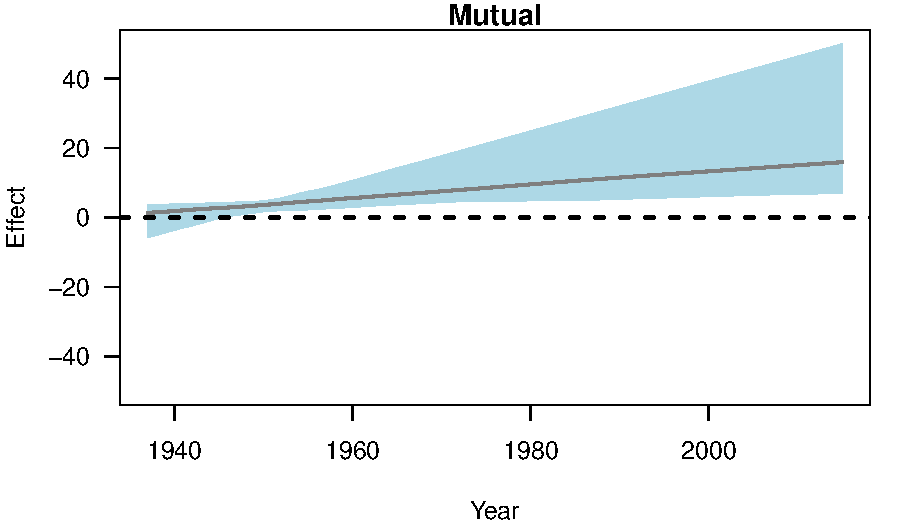
\includegraphics[width = 0.475\textwidth, trim= 0.1cm 1cm 0.5cm .45cm,clip=true]{images/mutual_coef_trend_linear.pdf} & 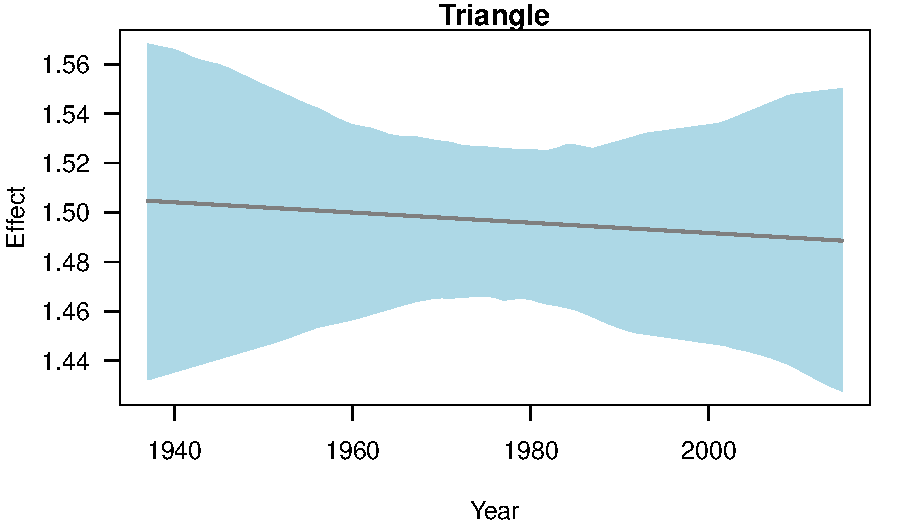
\includegraphics[width = 0.475\textwidth, trim= 0.1cm 1cm 0.5cm .45cm,clip=true]{images/triangle_coef_trend_linear.pdf} \\
 
%    (c) Activity & (d) Popularity \\
%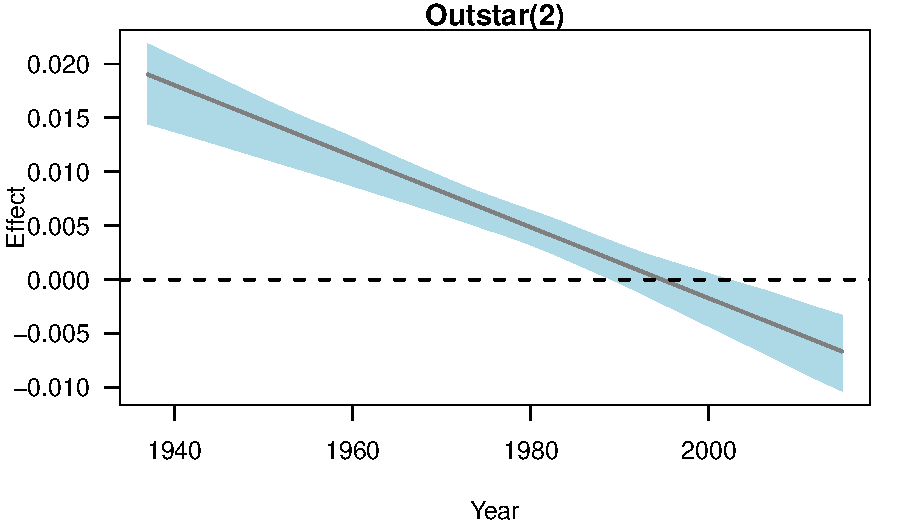
\includegraphics[width = 0.475\textwidth, trim= 0.1cm 1cm 0.5cm .45cm,clip=true]{images/o2star_coef_trend_linear.pdf} & 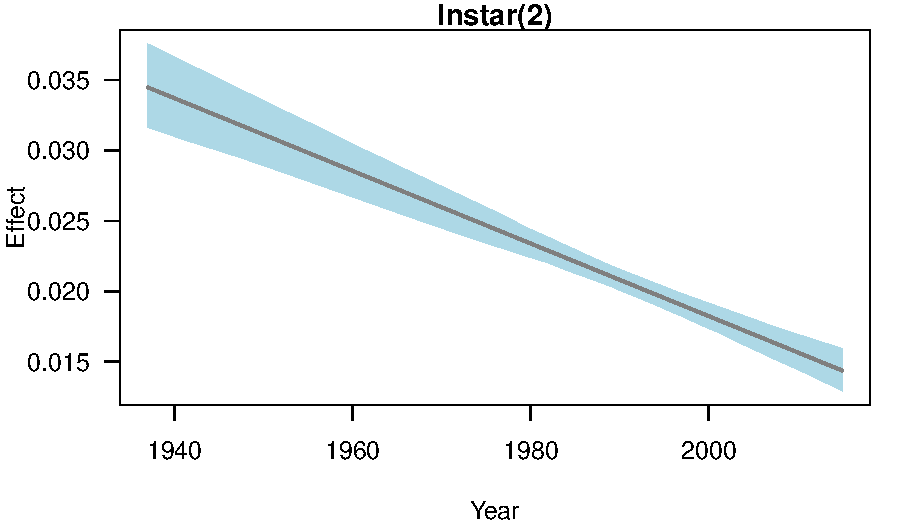
\includegraphics[width = 0.475\textwidth, trim= 0.1cm 1cm 0.5cm .45cm,clip=true]{images/i2star_coef_trend_linear.pdf} \\
 

 
%\end{tabular}
%\caption{Trending effects for dependence effect estimates from the c-TERGM. The solid lines plot the point estimates, and the shaded areas span 95\% confidence intervals. }
% \label{fig:coeftrends_endo}
%\vspace{-.25cm}
%\end{figure} 


%  \begin{figure}[H]
%  \begin{tabular}{cc}
% (e) MQ Score Difference & (f) Ideological Breadth \\
%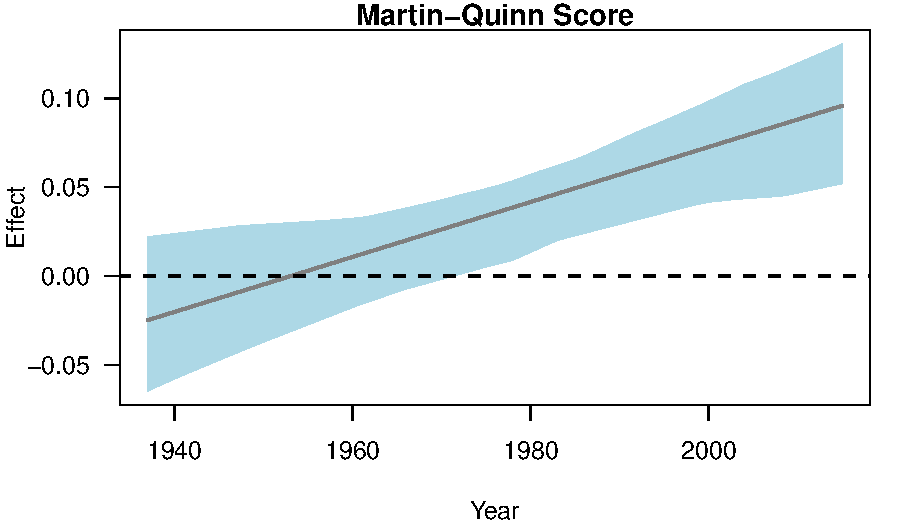
\includegraphics[width = 0.475\textwidth, trim= 0.1cm 1cm 0.5cm .45cm,clip=true]{images/mq_coef_trend_linear.pdf} & 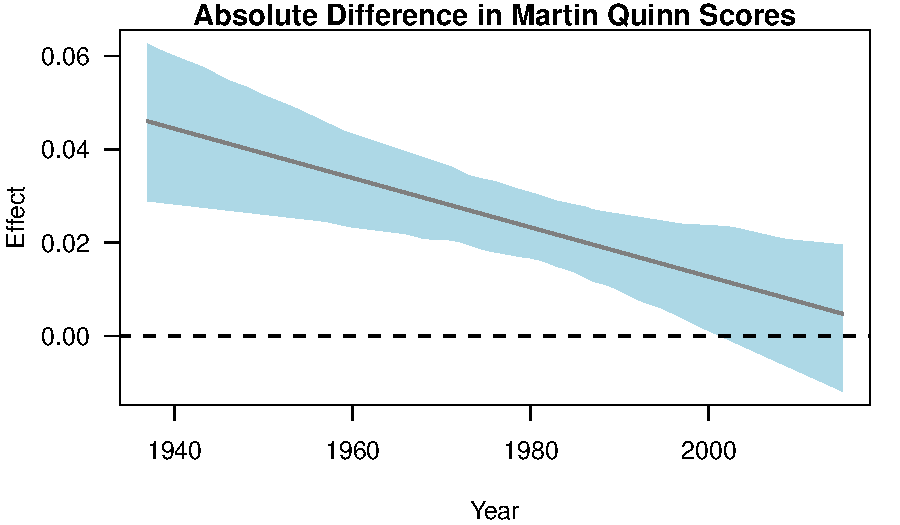
\includegraphics[width = 0.475\textwidth, trim= 0.1cm 1cm 0.5cm .45cm,clip=true]{images/absdiffmq_coef_trend_linear.pdf} \\
 
%  (g) Same Issue & (h) Majority Size \\
%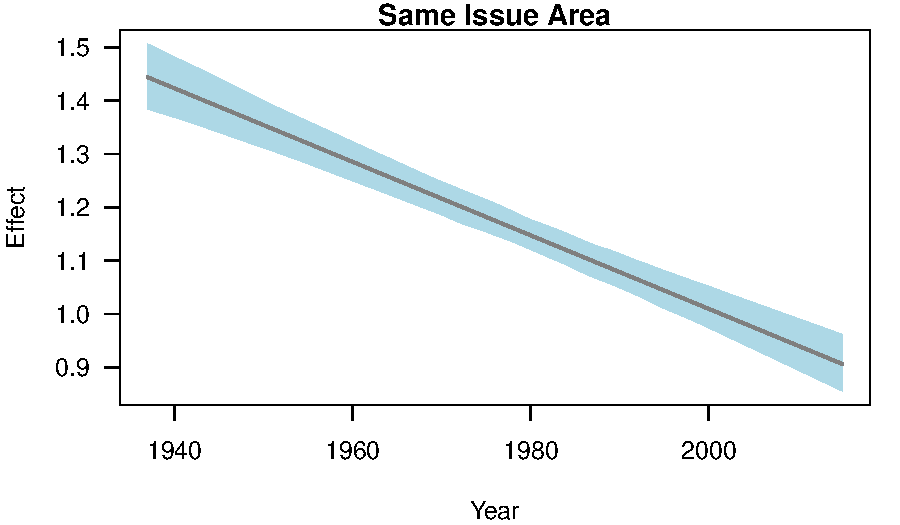
\includegraphics[width = 0.475\textwidth, trim= 0.1cm 1cm 0.5cm .45cm,clip=true]{images/sameissue_coef_trend_linear.pdf} & 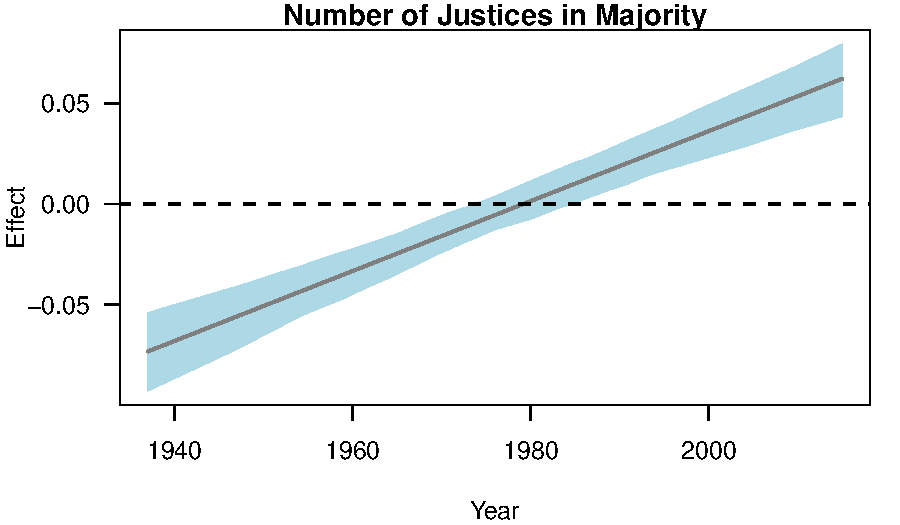
\includegraphics[width = 0.475\textwidth, trim= 0.1cm 1cm 0.5cm .45cm,clip=true]{images/numberjusticespro_coef_trend_linear.pdf} \\

% (i) Difference in Years & (j) Difference in Years$^2$ \\
%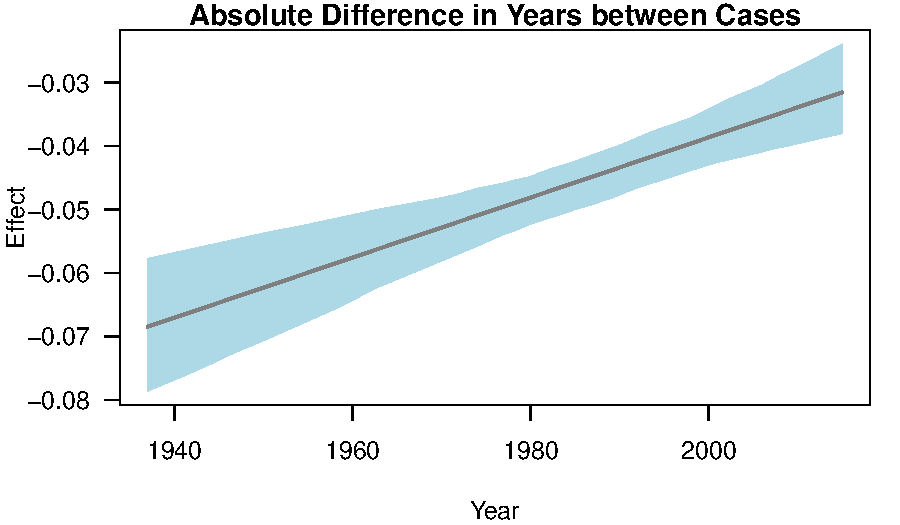
\includegraphics[width = 0.475\textwidth, trim= 0.1cm 1cm 0.5cm .45cm,clip=true]{images/yeardiff_coef_trend_linear.pdf} & 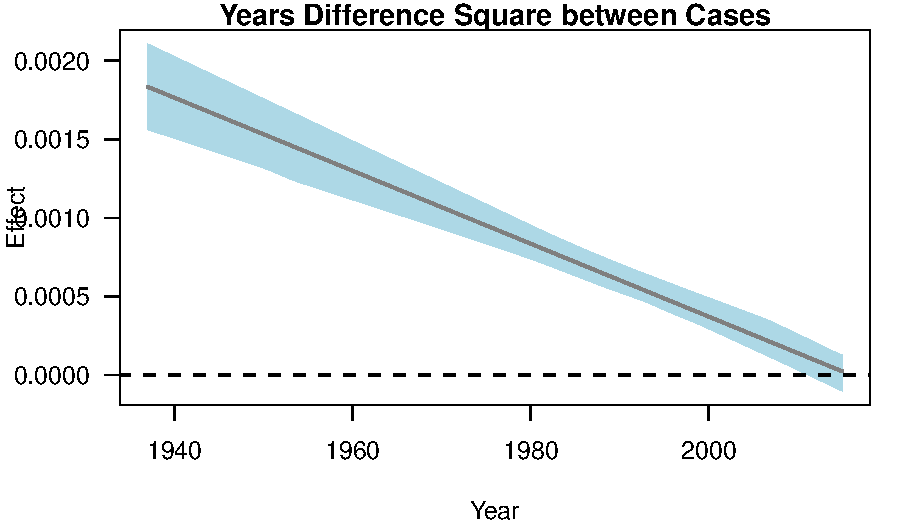
\includegraphics[width = 0.475\textwidth, trim= 0.1cm 1cm 0.5cm .45cm,clip=true]{images/yeardiffsquare_coef_trend_linear.pdf} \\

% (k) Overruled Cases & (l) Justice Homophily \\
%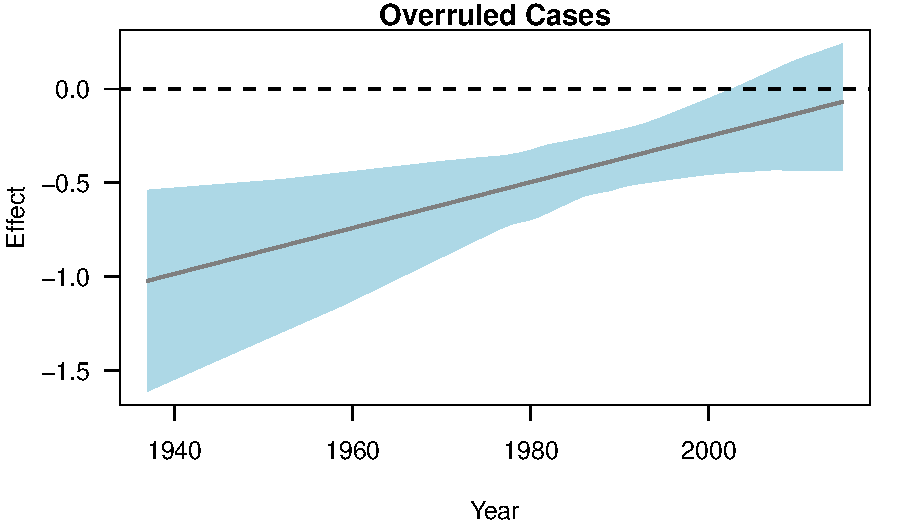
\includegraphics[width = 0.475\textwidth, trim= 0.1cm 1cm 0.5cm .45cm,clip=true]{images/overruled_coef_trend_linear.pdf} & 
%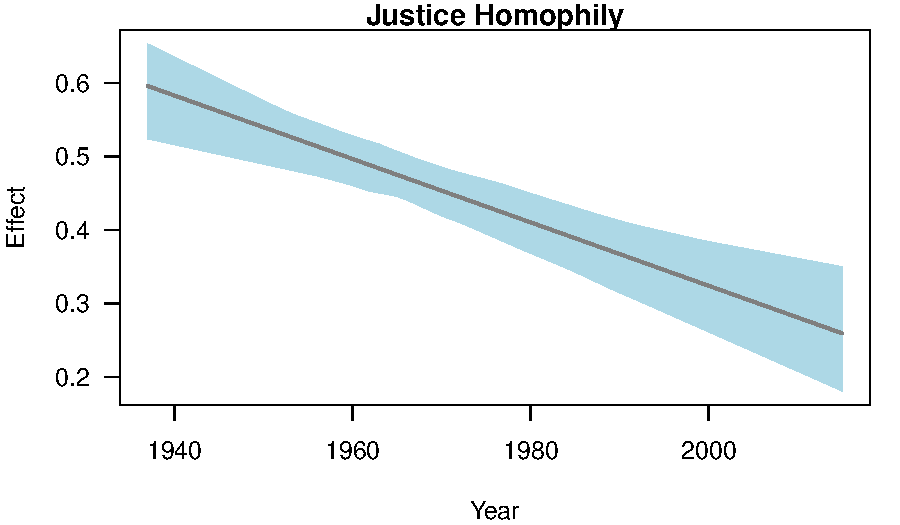
\includegraphics[width = 0.475\textwidth, trim= 0.1cm 1cm 0.5cm .45cm,clip=true]{images/justicehomophily_coef_trend_linear.pdf} \\

% \end{tabular}
%\caption{Trending effects for exogenous variables from the c-TERGM. The solid lines plot the point estimates, and the shaded areas span 95\% confidence intervals. }
% \label{fig:coeftrends_exo}
%\vspace{-.25cm}
%\end{figure} 


%\begin{itemize}
%\item visualize Sender/receiver Issue Area Results
%\item heatplot for issue area nodemix
%\item visualize Sender/receiver for majority opinion writer
%\item add Network effect plots for model without network statistics (add to existing plots?)
%\end{itemize}

%\newpage
%   \thispagestyle{empty}
   
   
  \begin{figure}[H]
\includegraphics[width=16cm]{SCC_Results_1}
\caption{ERGM results for the dependence terms. Circles indicate a p-value smaller than 0.05, squares a p-value between 0.05 and 0.1 and triangles a p-value greater than 0.1. }
 \label{SCC_results_1}

\vspace{-.25cm}
\end{figure}  


% \thispagestyle{empty}
 \begin{figure}[H]
\includegraphics[width=16cm]{SCC_Results_2}
\caption{ERGM results for the covariate terms. Circles indicate a p-value smaller than 0.05, squares a p-value between 0.05 and 0.1 and triangles a p-value greater than 0.1.}
 \label{SCC_results_2}
\vspace{-.25cm}
\end{figure} 




\section{Conclusion}

We present a methodology for studying citations between US Supreme Court opinions at the dyadic level, as a network. This methodology---the citation-ERGM---enables researchers to include both exogenous covariates such as the ideological predisposition and age of a case, and dependence terms, such as transitivity and reciprocity, as explanations for citation formation. We apply this methodology to a network that includes all Supreme Court cases decided between 1950 and 2015. We find, somewhat counterintuitively, that Supreme Court citations are highly reciprocal. We also find that citations are driven by dependencies such as triad closure and popularity. The dependence effects that we identify are as substantively and statistically significant as the effects of the exogenous covariates we include in the model. The summary result from this analysis is that theoretical models of Supreme Court citation formation should consider both the effects of case characteristics and the structure of past citations. 

%We recognize two important limitations of the current analysis, which should be addressed in future iterations of this work or in future studies. First, our theoretical claims and analyses treat all citations---positive and negative---as equivalent. Both data and methodological limitations will need to be overcome to consider these two citation types. Second, there is nothing in the c-ERGM that governs the generation of new cases (i.e., cases are assumed to arise exogenously, unrelated to the history of the citation network). As new cases are often taken up by the Supreme Court in order to test, clarify, and/or challenge existing precedents, it is likely inappropriate to assume that new cases arise exogenous to the existing citation network. Overcoming this limitation would require methodological innovation in the c-ERGM as well as theoretical development regarding exactly how citation structure might predict case emergence. 
 



\bibliography{bib} 
\bibliographystyle{apsr}




\end{document}





















